\begin{figure}[h]
    \centering
    % Top figure
    \begin{subfigure}[b]{\textwidth}
        \centering
        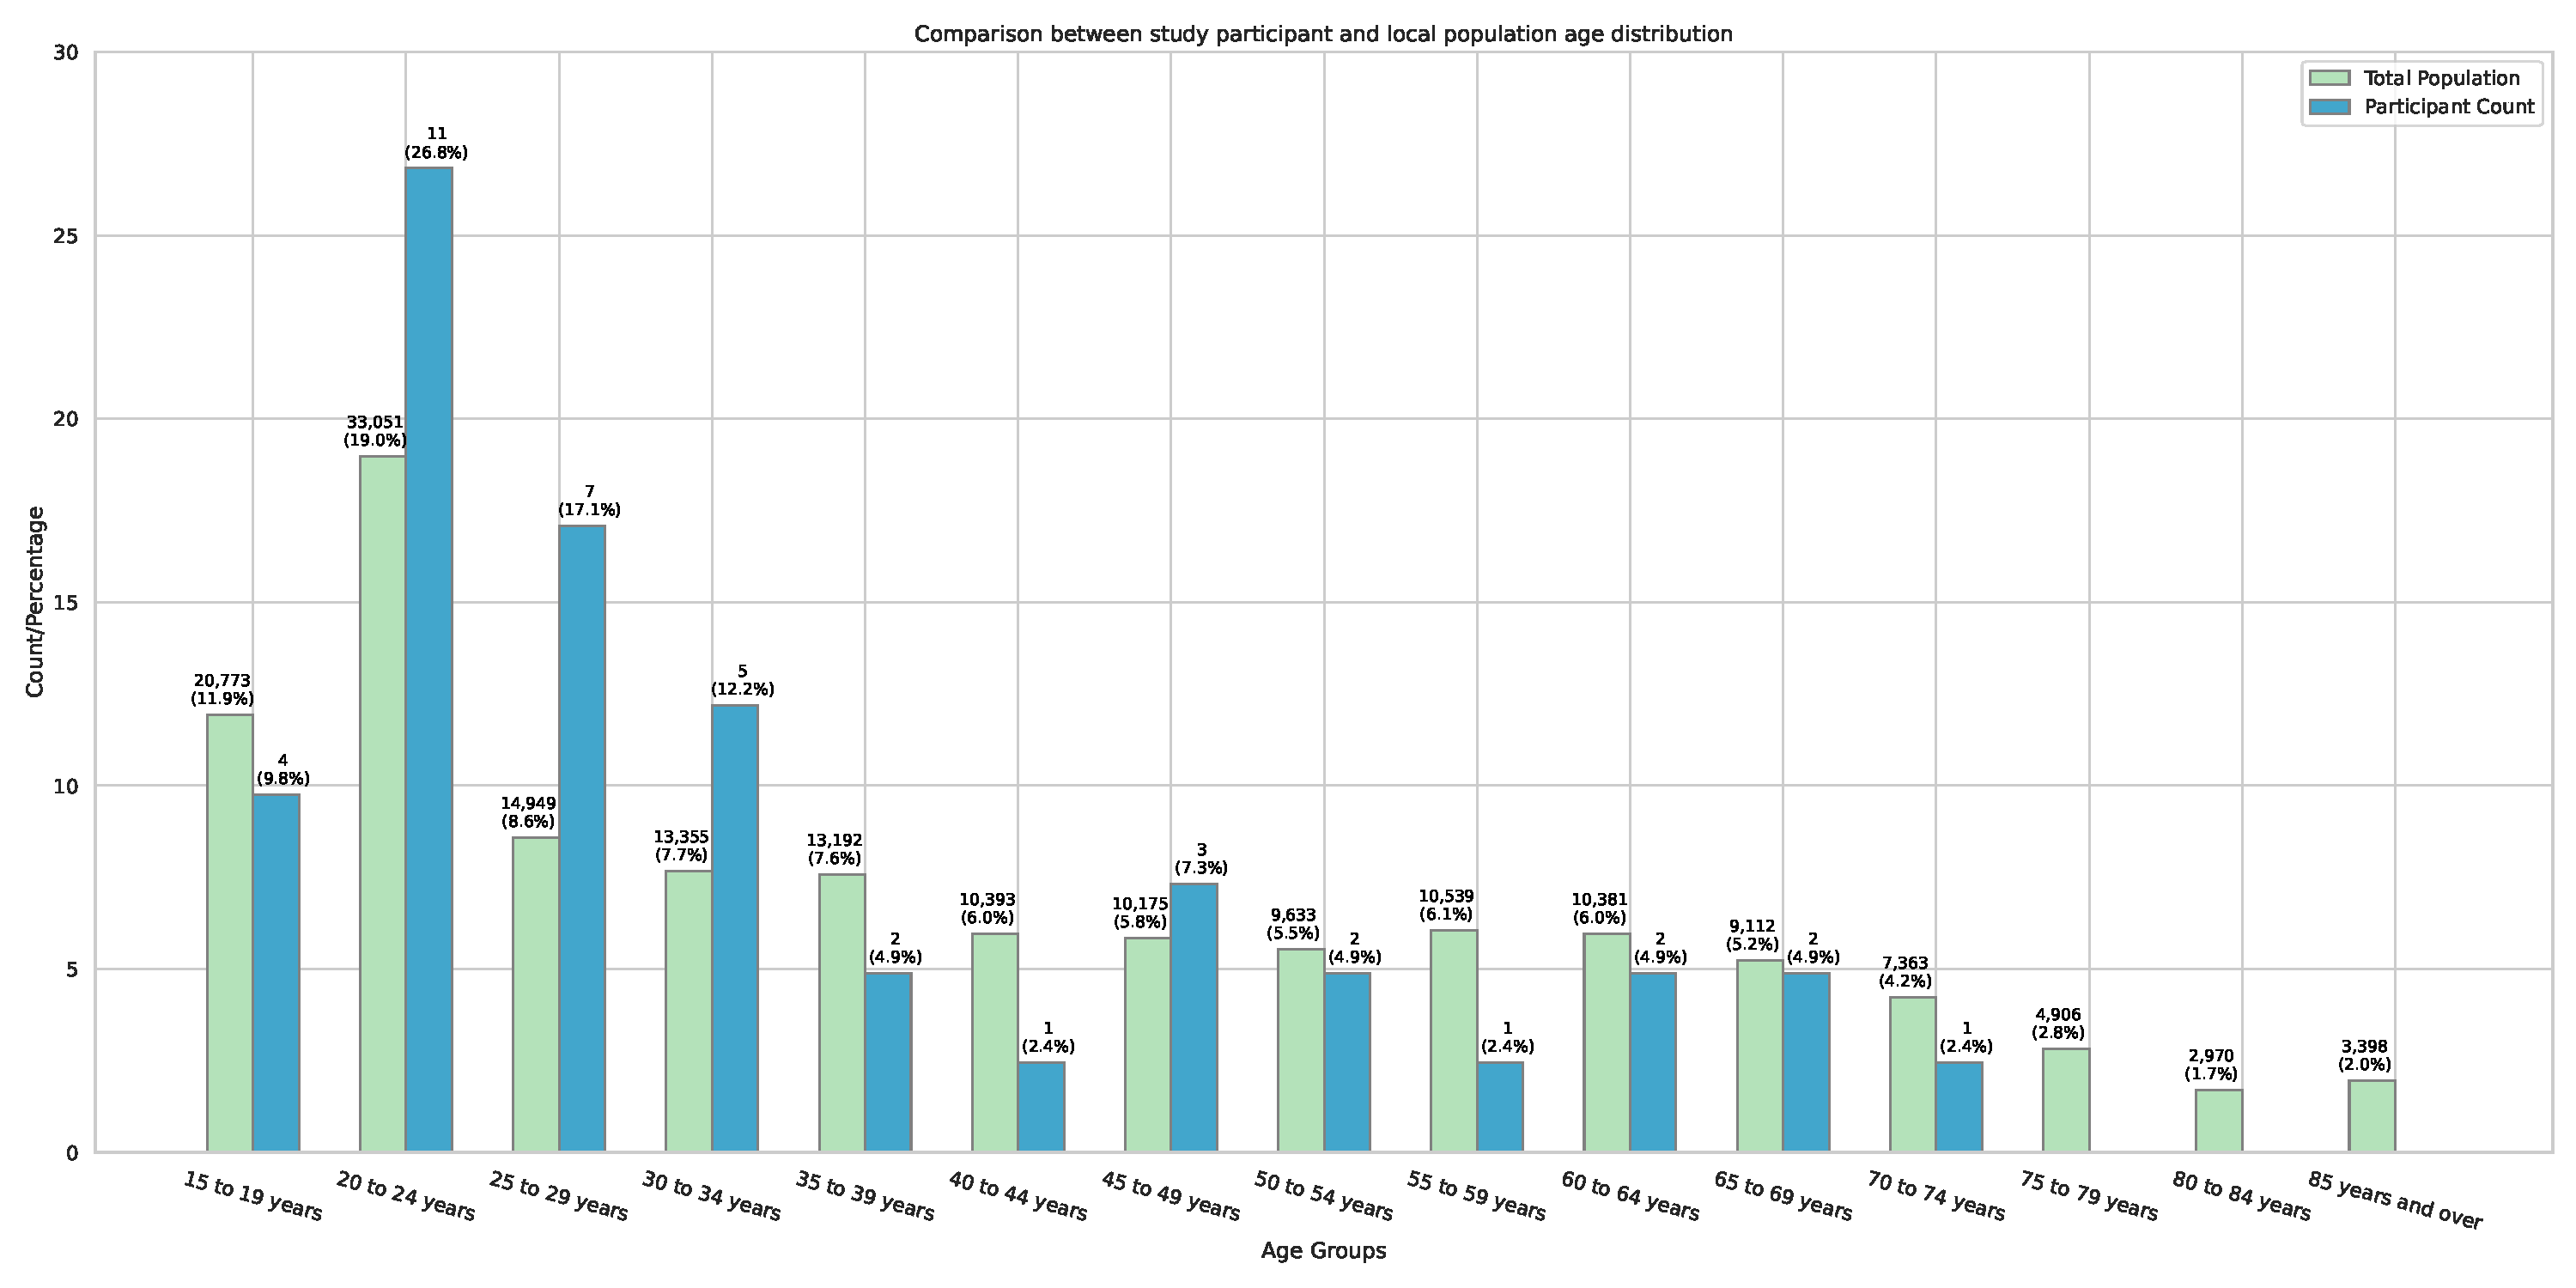
\includegraphics[width=\textwidth]{content/image/demo/demo_age_group_vertical.pdf}
        \caption{Age distribution}
        \label{fig:demoAge}
    \end{subfigure}
    
    \vspace{0.5cm} % Add some vertical space between the rows

    % Bottom figures
    \begin{subfigure}[b]{0.45\textwidth}
        \centering
        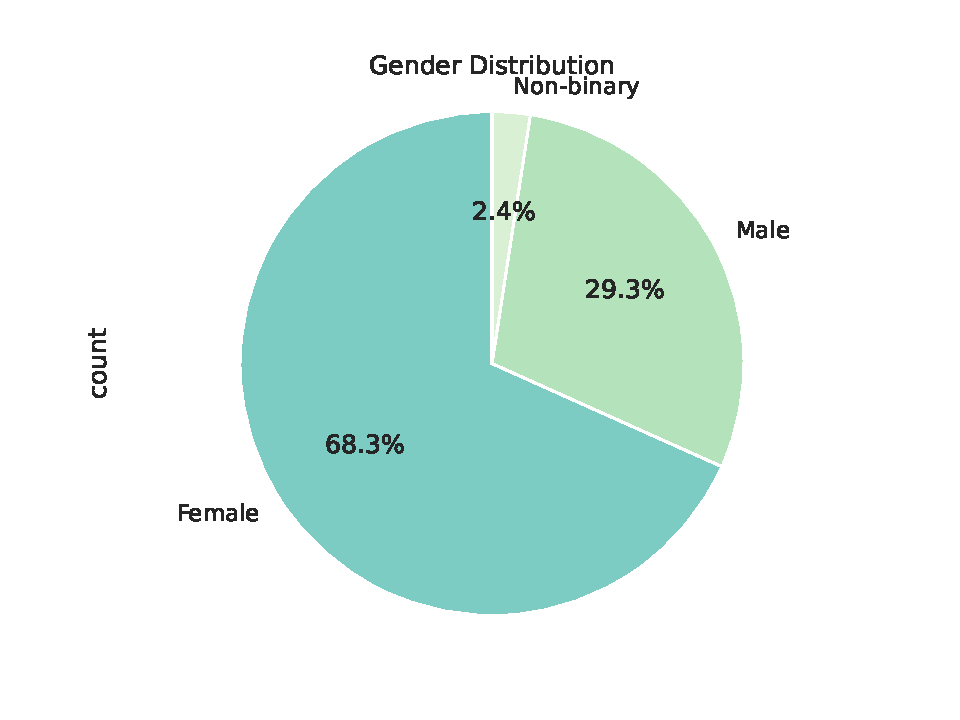
\includegraphics[width=\textwidth]{content/image/demo/demo_gender.pdf}
        \caption{Gender distribution}
        \label{fig:demoGender}
    \end{subfigure}
    \hfill
    \begin{subfigure}[b]{0.45\textwidth}
        \centering
        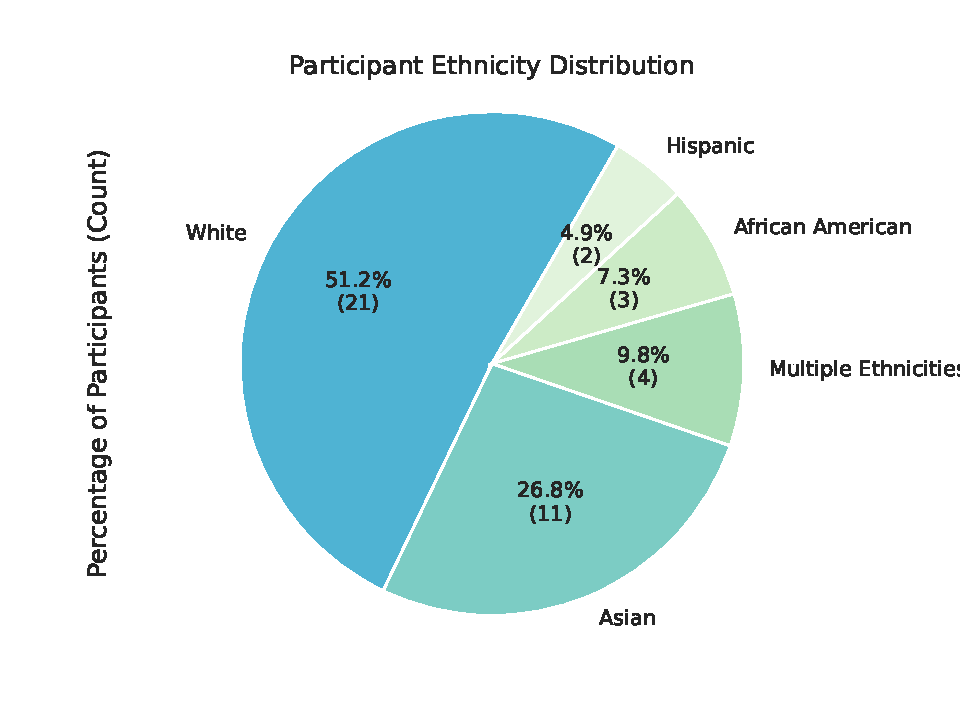
\includegraphics[width=\textwidth]{content/image/demo/demo_ethnicity.pdf}
        \caption{Ethnicity distribution}
        \label{fig:demoEthnicity}
    \end{subfigure}
    
    \caption{Demographic distributions: Age, Gender, and Ethnicity}
    \label{fig:Demographics}
\end{figure}

% maybe more the figure to the appendix?
\section{Cognitive Load and Sources across Experiment Conditions}
\label{sec:cog_result}
In this section, we present the cognitive load across experiment groups and the sources contributing to each cognitive load dimension. Given the limited number of participants, we focus on descriptive statistics and qualitative assessments of cognitive load. Quantitative data includes metrics from the survey tasks, while qualitative insights come from post-survey interviews transcribed and analyzed by the first author.

To analyze the qualitative data, the first author conducted an inductive thematic analysis process~\cite{olsonWaysKnowingHCI2014}. They coded snippets from each transcript based on specific research questions and topics of interest for the qualitative analysis. Similar codes were merged within each research question or topic to form relevant themes. When differences were hypothesized, they applied a deductive coding process to text snippets related to a specific research question or topic of interest.

The results for this section are organized as follows: We start with participant demographics and then provide an overview of our cognitive load findings. We then examine the six dimensions used in the NASA-TLX survey: mental demand, physical demand, temporal demand, performance, effort, and frustration.

\subsection{Demographics}
We recruited a total of $41$ participants, allocating ten to each experiment condition. Due to data quality concerns, we excluded one participant's data\footnote{The participant stated they believed the experiment as a fake setup that they did not need to complete seriously.}. The mean age of the participants was $34.63$ years old, with a detailed age distribution presented alongside the county population distribution in Figure~\ref{fig:demoAge}. This comparison reveals that our sample closely matches the county's demographic profile, albeit with a slightly higher representation of younger adults, particularly in the 35-45 age range. As shown in Figure~\ref{fig:demoGender}, the majority of participants skewed toward females.

Regarding ethnicity, $51.2\%$ of the participants identified as White, $26.8\%$ as Asian, $7.3\%$ as African American, and $4.9\%$ as Hispanic. Additionally, $9.8\%$ of participants reported mixed ethnicity.

\subsection{Overall Cognitive Load}
\label{sec:cog}
\begin{figure}[ht]
    \centering
    \begin{subfigure}[b]{0.45\textwidth}
        \centering
        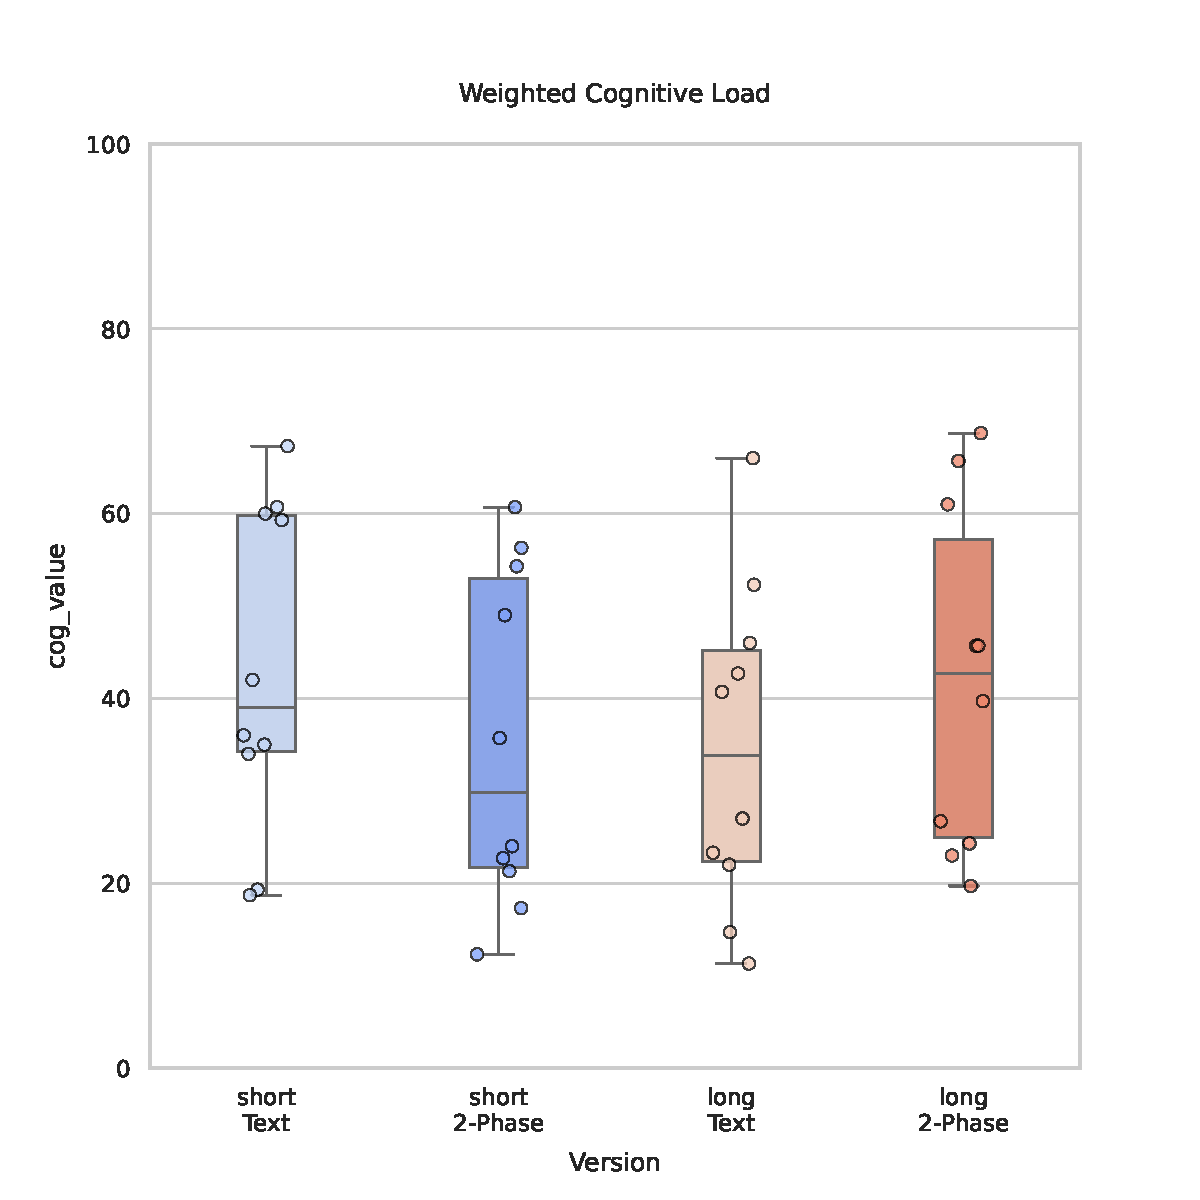
\includegraphics[width=\textwidth]{content/image/results/nasatlx_final_value.pdf}
        \caption{NASA-TLX Weight Score Distribution}
        \label{fig:nasatlx-final1}
    \end{subfigure}
    \hfill
    \begin{subfigure}[b]{0.47\textwidth}
        \centering
        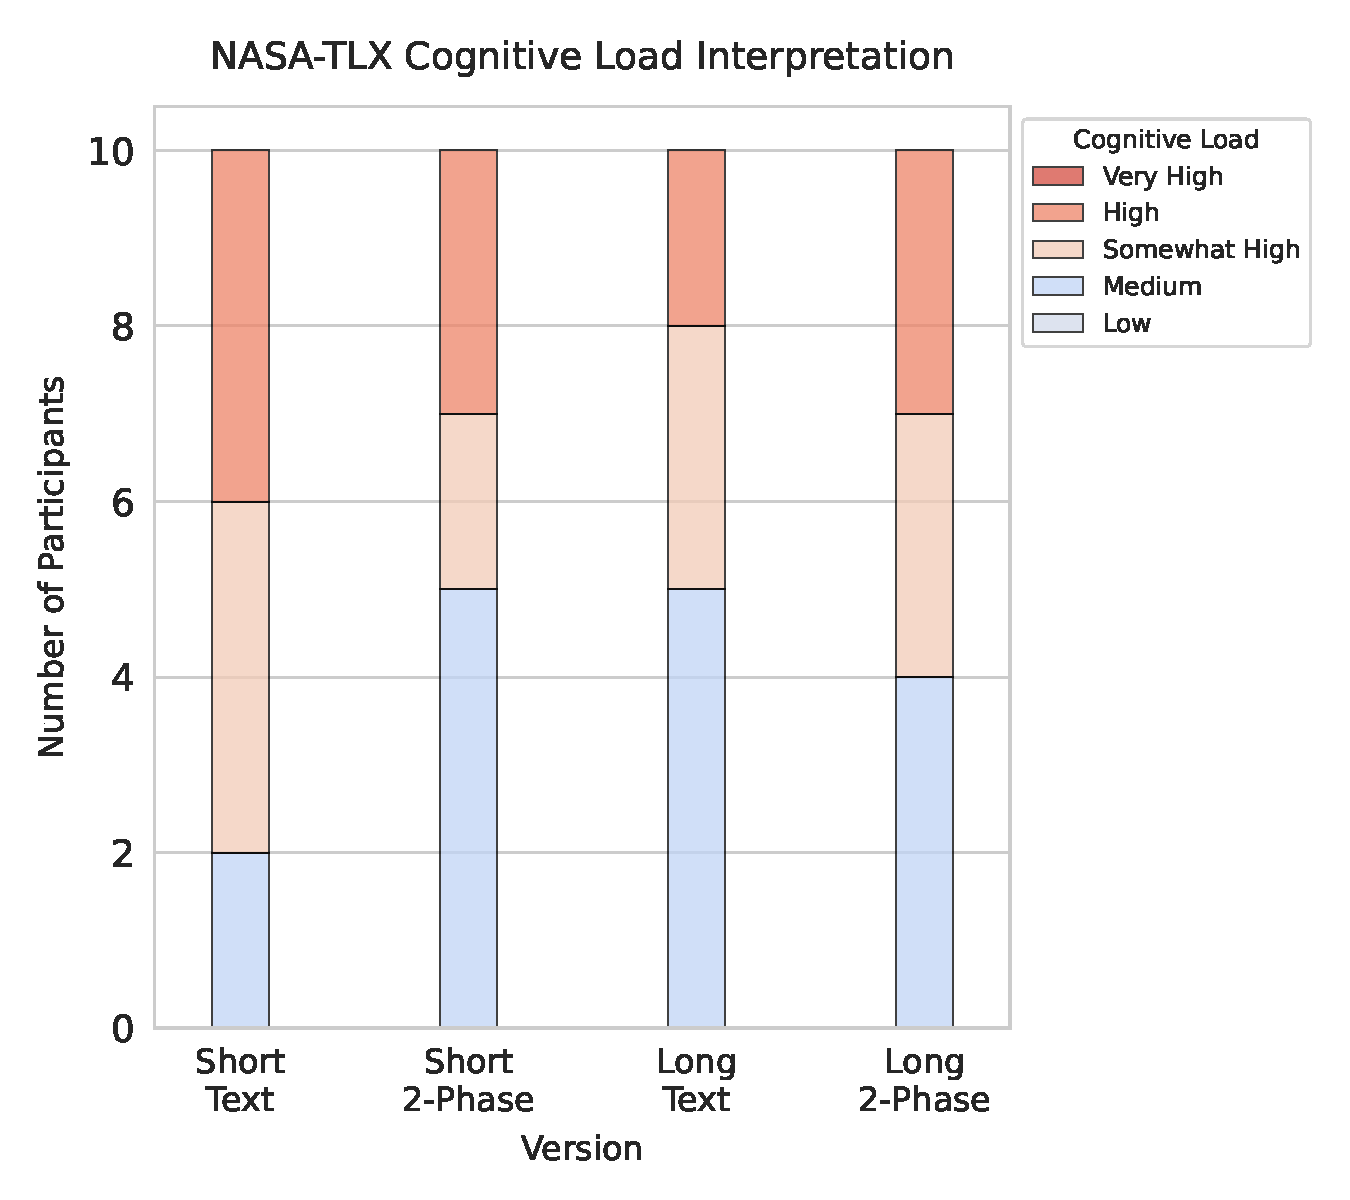
\includegraphics[width=\textwidth]{content/image/results/nasatlx_cog_value_interpreted.pdf}
        \caption{NASA-TLX Cognitive Interpretation}
        \label{fig:nasatlx-final2}
    \end{subfigure}
    \caption{This figure shows the box plot results for weighted NASA-TLX scores across experiment groups and participant counts based on individual score interpretations. In~\ref{fig:nasatlx-final1}, we observe a downward trend in cognitive load for the short QS, while the long QS shows an upward trend. Interestingly, there is a counterintuitive downward trend between short and long text interfaces. In~\ref{fig:nasatlx-final2}, these trends are clearer when NASA-TLX scores are grouped into five tiers.}
    \label{fig:nasatlx-final}
\end{figure}

To answer~\textbf{RQ1} and~\textbf{RQ2a}, we derive the weighted NASA-TLX scores across the four experiment conditions. We show these results in Figure~\ref{fig:nasatlx-final}. Weighted NASA-TLX uses a continuous 0-100 score, with higher values indicating greater cognitive load. We use predefined mappings of NASA-TLX values to cognitive levels: low, medium, somewhat high, high, and very high, as listed by~\textcite{hart1988development}. We show value interpretations in Figure~\ref{fig:nasatlx-final2}. We find that:

\begin{itemize}
    \item Short text interface: The median cognitive load was $39.00$, with a mean of $43.23$ and a standard deviation of $17.65$. $8$ participants reported somewhat high or above, with $4$ reporting high cognitive load.
    \item Short interactive interface: The median cognitive load was $29.85$, with a mean of $35.36$ and a standard deviation of $18.17$. $5$ participants reported somewhat high or above, with $3$ reporting high cognitive load.
    \item Long text interface: The median cognitive load was $33.85$, with a mean of $34.60$ and a standard deviation of $17.69$. $5$ participants reported somewhat high or above, with $2$ reporting high cognitive load.
    \item Long interactive interface: The median cognitive load was $42.70$, with a mean of $42.02$ and a standard deviation of $18.48$. $6$ participants reported somewhat high or above, with $3$ reporting high cognitive load.
\end{itemize}

These results partially answer our first two research questions. First, across the short survey, the interactive interface decreased cognitive load compared to the text interface. This is evident from the median cognitive load decrease from $39.00$ to $29.85$, with more participants reporting lower cognitive load using the interactive interface. The short text interface had the most participants ($N=8$) rating their cognitive load as somewhat high or above. The other three conditions had similar distributions, with about half experiencing medium and half somewhat high or high loads.

Second, contrary to our expectations, the long text interface had a lower cognitive load than the long interactive interface. The cognitive load for the long text interface was even lower than that for the short text interface, with a median cognitive load of $33.85$ compared to $39.00$ in the short text interface. This is counterintuitive, as prior literature suggests that more options can heighten cognitive load~\cite{swellerCognitiveLoadTheory2011}.

By deduction, if the interactive interface increased cognitive load in the long survey, we might expect a similar increase in the short interactive interface compared to the short text interface. However, we observed a lower cognitive load in the short interactive interface. This discrepancy suggests two plausible explanations:

\paragraph{Interactive Interface prevents satisficing from cognitive overload} The long survey leads to cognitive overload and encouragesd satisficing behaviors, but the interactive components may have prevented participants from taking these mental shortcuts, which would typically reduce measured cognitive load~\cite{daniel2017thinking, simonBehavioralModelRational1955, payneAdaptiveStrategySelection1988, tverskyJudgmentsRepresentativeness}. This prevention could result in a higher cognitive load in the long interactive interface compared to the long text interface. In other words, the interactive interface may have shifted participants' cognitive load from some dimensions to others, maintaining their overall cognitive load at a higher level but not overloaded. If this is true, we expect to see differences among the qualitative explanations of sources, specifically differences in the perceived causes of cognitive load. We will explore this in the next subsections (Subsections~\ref{sec:mental}-\ref{sec:fustration}).

\paragraph{A Pure Increase of Cognitive Load Due to Interactivity} It is also possible that the long survey introduced statisficing behaviors due to cognitive overload, and the interactive interface did not influence participants' preference construction but only increased cognitive load due to the added interactivity. In other words, participants are asked to perform additional operations with interactive elements that contribute to a higher cognitive load without providing sufficient cognitive benefits. If this is true, we should expect behavior data to show similar voting patterns across conditions, as the added interactions primarily focused on the pre-organization of the options rather than influencing the decision-making process itself. We will explore this in the section~\ref{sec:behave_result}.

We also acknowledge the possibility that the elicited values are pure noise and do not reflect the actual cognitive load. This could be due to the small sample size, the nature of the task, or the participants' understanding of the cognitive load scale. While this might be true for small sample sizes, we believe that the qualitative insights from the interviews provide a more nuanced understanding of the cognitive load sources. We detail these limitations in Section~\ref{sec:limitations}.

% ============================================= %
\begin{table}[h]
    \caption{This table lists all the causes participants mentioned as contributing to their Mental Demand. The shaded cells represent the percentage of participants citing each source of mental demand, allowing for comparison within columns. The abbreviations are: ST (Short Text Interface), SI (Short Interactive Interface), LT (Long Text Interface), and LI (Long Interactive Interface). Short and Long refer to the sum across both interfaces; Text and Inter refer to the sum across both survey lengths. We include Sparklines for comparisons across these experiment groups.}
    \label{tbl:mental}
    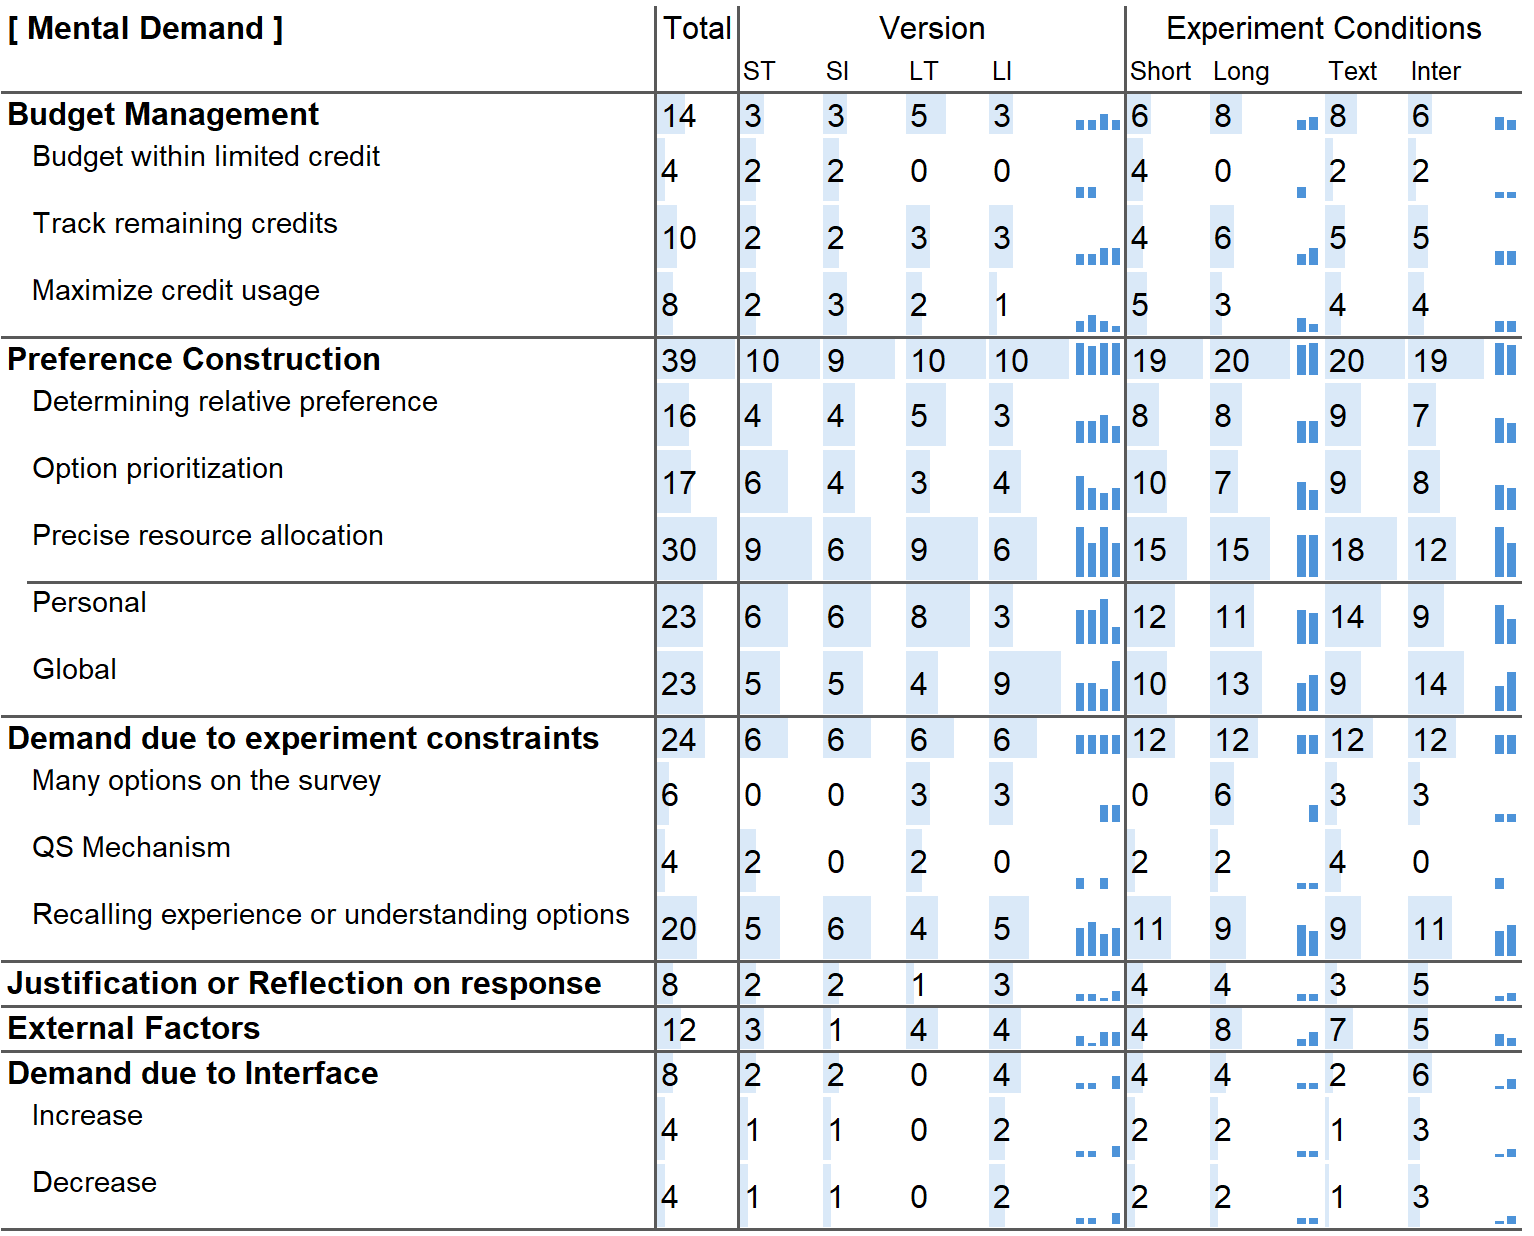
\includegraphics[width=\linewidth]{content/image/cog/mental_table.png}
\end{table}
\subsection{Source of Mental Demand}
\label{sec:mental}

\vspace{5pt}
\begin{tldrbox}
    \faInfoCircle~\xspace\textbf{Summary:} Participants across all groups highlighted~\textbf{budget management} and~\textbf{preference construction} as their primary sources of mental demand. We observed two key differences: First, slightly more participants using the text interface reported mental demand from precisely determining the number of votes for options compared to the interactive interface. Second, when it comes to long QS, participants using the long interactive interface considered broader societal impacts and evaluated options holistically, while those in the long text interface focused on personal relevance and individual issues. These differences indicate that the interactive interface encouraged deeper thinking, shifting the source of mental demand. % We find evidence that the interactive interface prevented cognitive overload.
\end{tldrbox}

Mental demand refers to the extent of mental and perceptual activity required. Interview results showed the top two causes that increased participants' mental demand were~\textit{Budget management} and~\textit{Preference construction}. Table~\ref{tbl:mental} listed all causes. We discuss in detail below.

Fourteen participants expressed demand from budgeting within limited credit (N=4), tracking remaining credits (N=10), and maximizing credit use (N=8). For example:

\subsubsection{Mental Demand Source: Budget management} $14$ participants expressed demand from budgeting within limited credit ($N=4$), tracking remaining credits ($N=10$), and maximizing credit use ($N=8$). For example:

\begin{displayquote}
How many I got left that~\ldots\ that I haven't voted on yet, and seeing if I and looking at the remaining credits, I'm trying to mentally divide that up before I start allocating upvotes and downvotes.

\small{\noindent \hfill -- S006, long interactive interface, budget within limited credit}
\end{displayquote}

\begin{displayquote}
And then I just wanted to make sure that I used all the credit that I had available to me, and also knowing that in order to like show your support for certain societal issues you had to like that was giving a tangential take away from other societal issues that you could support as well.
    
\noindent \hfill -- S032, short text interface, track remaining credits.
\end{displayquote}

In the first quote, the participant struggles with not running out of credit while allocating credits. The second quote highlights the challenge of maximizing spend while ensuring sufficient differentiation. Both relate to effective budget management.

We further categorized budget management causes as operational (completing an operation, e.g., using the last credit) or strategic (achieving a higher goal, e.g., spreading credits across options). Strategic planning does not refer to gaming out others or 'winning' a game but rather to high-level thinking processes that consider strategies and plans to tackle a challenge, compared to operational tasks such as adjusting a specific vote value. Most long survey participants reported operational causes, indicating they didn't face enough mental demand to consider additional strategies.

\subsubsection{Mental Demand Source: Preference construction}
Almost all participants ($N=39$) reported increased mental demand from preference construction. We broken it down into three sources: determining relative preference ($N=16$), option prioritization ($N=17$), and precise resource allocation ($N=30$), For example, participants would focus on internal evaluation and construct comparisons among different options:

\begin{displayquote}
Figuring out my priorities, and how much I prioritize option 1 over option 2. What is the difference between those 2 on my priority list?

\hfill -- S002, short interactive interface, determining relative preference
\end{displayquote}

% I think the whole time I was trying to balance, I think II think I partly was discovering my what's the word I want to use bias isn't quite right. My priorities (S031, I)

Participants would locate higher priority options through trade-off decision making or map existing internal preferences into a subset of options:

\begin{displayquote}
I knew which ones that I wanted to dedicate the most to, and I knew which one I wanted to dedicate the least to. But it was that middle area that was kind of a grey area.
    
\noindent \hfill -- S008, short interactive interface, option prioritization
\end{displayquote}

% I knew which ones that I wanted to dedicate the most to, and I knew which one I wanted to dedicate the least to. But it was that middle area that was kind of a grey area.
% \noindent \hfill -- S024, short text interface, option prioritization

Finally, participants tried to allocate specific values or make specific 
adjustments to represent their preferences. 

\begin{displayquote}
I'm not sure how to put into words~\ldots like having to pick how many upvotes would go to each one
    
\noindent \hfill -- S023, long text interface, precice resource allocation
\end{displayquote}

Almost all participants mentioned preference construction as a source of mental demand, supporting the theory that preference construction is a difficult and mentally demanding task. Notably, more participants using the text interface reported mental demand from precise resource allocation compared to the interactive interface ($18$ vs. $12$). We conjecture that the interactive interface helped participants make more informed decisions, reducing their mental demands in this area.


\subsubsection{Mental Demand Source: Other Sources}
We identified four additional sources causing participants' mental demands: \textit{experiment setup}, \textit{number of options}, \textit{QS mechanism}, and \textit{external factors}. 

$24$ participants mentioned the experiment setup mainly related to understanding and recalling their experience with the options. $6$ participants, all from the long QS, found the number of options added mental demand. $4$ participants cited working with getting familiar with the QS mechanism as a source of mental demand. These are sources related to the study design. $12$ participants mentioned external factors, such as considering the consequences of their results or the challenges decision-makers face. $4$ participants reported an increase and another four a reduction in mental demand due to the interface design. $8$ participants expressed mental demand from justifying their choices and reflecting on their responses, questioning whether their votes truly reflected their preferences or if the amount of credit spent was justified.

\subsubsection{Takeaway: A different scope of preference construction and budget management approach among long QS groups}
\label{sec:mental_takeaway}

While these sources are common across all experiment groups, we highlight a notable difference when we focus on participants across interfaces completing the long QS. \textbf{They focus on a different scope of preference construction}. More specifically, participants ($N=8$) in the long text interface tend to experience mental demand from preference construction by thinking about issues more narrowly and focusing on personal relevance. Conversely, participants ($N=9$) in the long interactive interface experience higher mental demand from considering the broader societal impact and evaluating options more comprehensively. Only four participants in the long text interface expressed a comprehensive view, and three participants in the long interactive interface expressed a narrow and personal view.

% \begin{displayquote}
% \bracketellipsis also seeing the long list and obviously having to pick between quite a few things that I do feel very strongly about and having to figure out which ones do, I feel more strongly about than others.
    
% \noindent \hfill -- S023, long text interface
% \end{displayquote}

\begin{displayquote}
Trying to figure out what upvotes I should give it you know~\ldots compared to~\ldots I even kind of went back compared to the other topics: <topic one> compared to <topic two>, and even with like <topic three>, I kind of went back and forth between those two. \bracketellipsis So it was very mental tasking for me.

\noindent \hfill -- S015, long text interface
\end{displayquote}

% \begin{displayquote}
% \bracketellipsis really having to think, especially with so many different societal issues. How do I personally prioritize them? And to what extent do I prioritize them?
    
% \noindent \hfill -- S009, long interactive interface
% \end{displayquote}

\begin{displayquote}
\bracketellipsis really going through the rest of the categories and deciding okay, which are the pressing issues of our time and which are the pressing issues for this particular society that that I live in. \bracketellipsis You know these causes need a lot more funding, and and others can probably still have some sort of an impact, even with less resources.

\noindent \hfill -- S019, long interactive interface
\end{displayquote}

In the first quote, participants felt mental demand focusing on three options, trying to recall specific characteristics to differentiate them. In the second quote, participants considered the societal impact of options, aiming to maximize their effect. This difference highlighted our belief that the organization phase prompted participants to consider a broader range of factors in their decisions. Across both interfaces, participants in the long survey tended towards operational mental demands related to budget management. We argue the interactive interface prevented participants from using heuristics to narrow their choices, which only appeared when final votes were determined, an area with less support from the interface. We conclude the interactive interface scaffolded the decision-making process, preventing satisficing behaviors because of cognitive overload, and thus shifted mental demand sources. This shift explains why we did not notice significant differences in mental demand raw values (Figure~\ref{fig:mental_cog_score}) across the four experiment groups.

% In addition, we also find that long text interface participants focused on more operational behaviors such as:

% \begin{displayquote}
% So I wanted to be fair.~\bracketellipsis I actually took my calculator out and said~\bracketellipsis  how much would it be if I equally distributed it and then how do I do that? Do I wanna do it all equally or not?

% \noindent \hfill -- S020, long text interface
% \end{displayquote}

% compared to more procedures involving more strategic planning such as:

% \begin{displayquote}
% I wanted to make sure I wanted to give some credit to everything~\bracketellipsis I'm trying to make sure that I had without doing a lot of~\ldots I guess redos is trying to kind of get it right the first time on how I weight things.

% \noindent \hfill -- S032, long interactive interface
% \end{displayquote}



% IN_T4: Wanting more information on the options (N=6/40)
% 5. While the numbers seem small, non of this request came from v3. This could explain that participants are already overloaded from the existing the task.

\begin{figure}[h]
    \begin{minipage}[t]{0.45\textwidth}
        \centering
        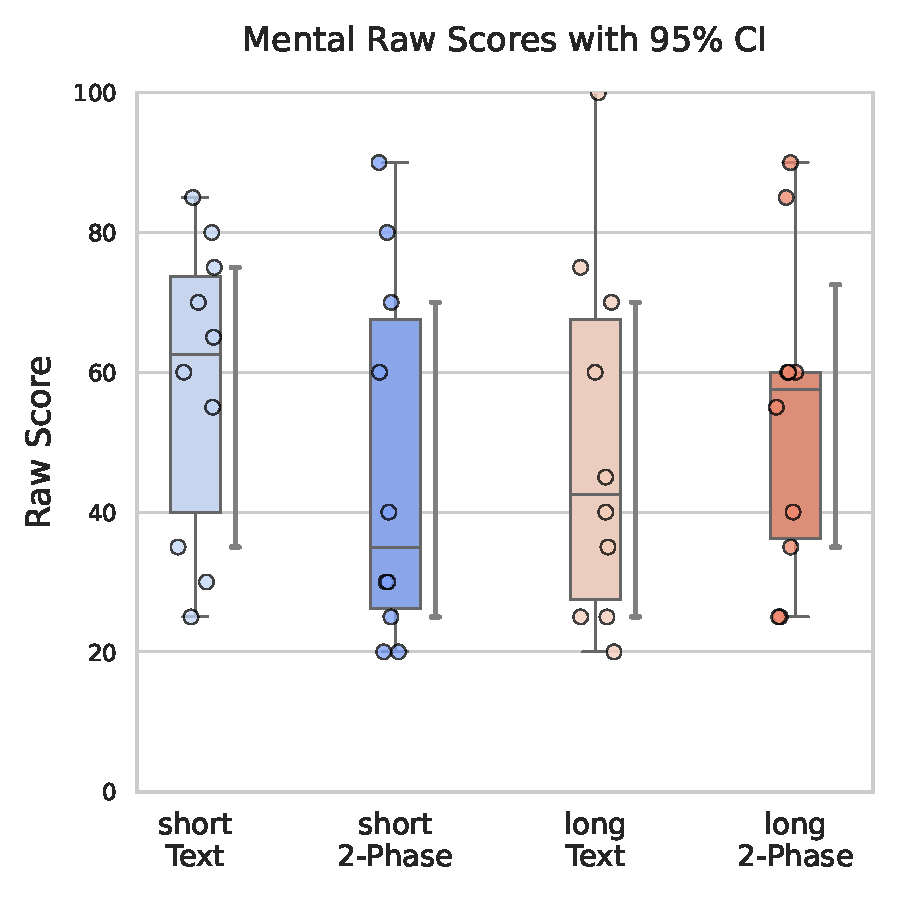
\includegraphics[width=\textwidth, trim=0 13 0 13, clip]{content/image/cog/Mental_scores.pdf}
        \captionsetup{width=0.9\textwidth, justification=justified}
        \caption{Mental Demand Raw Score: Across all four experiment groups, participants' reported mental demand is spread across a wide range with many participants experiencing high mental demand.}
        \label{fig:mental_cog_score}
    \end{minipage}
    \hfill
    \begin{minipage}[t]{0.45\textwidth}
        \centering
        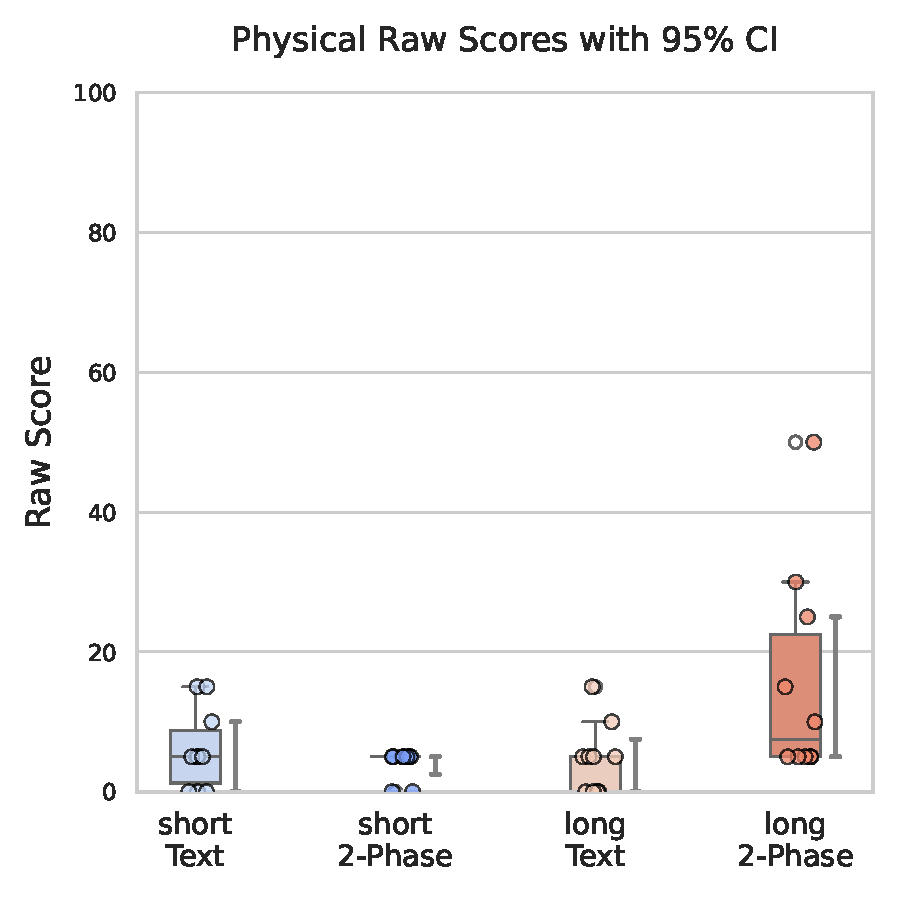
\includegraphics[width=\textwidth, trim=0 13 0 13, clip]{content/image/cog/Physical_scores.pdf}
        \captionsetup{width=0.9\textwidth, justification=justified}
        \caption{Physical Demand Raw Score: Participants other than the long interactive interface reported minimal physical demand. The long interactive interface had the highest physical demand, likely due to increased mouse clicks and extended time spent looking at the vertical screen.}
        \label{fig:physical_cog_score}
    \end{minipage}
\end{figure}

% ============================================= %
\begin{table}[h]
    \caption{Physical Demand Causes: Most participants expressed little or no physical demand. Results reflected that participants in the long interactive interface required more actions, hence the higher mention of mouse usage as a source.}
    \label{tbl:physical}
    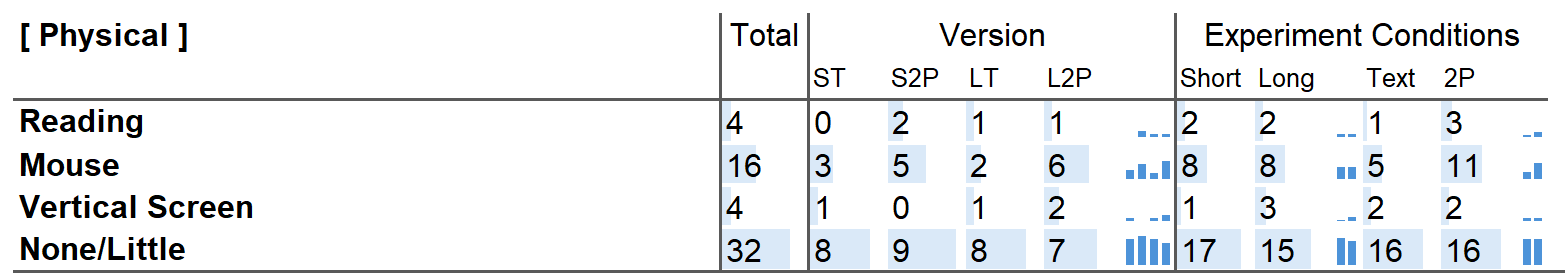
\includegraphics[width=\linewidth]{content/image/cog/physical_table.png}
\end{table}

\subsection{Source of Physical Demand} 
\label{sec:physical}

\vspace{5pt}
\begin{tldrbox}
    \faInfoCircle~\xspace\textbf{Summary:} Participants across all groups highlighted \textit{reading}, \textit{using the mouse}, and \textit{navigating a vertical screen} as cause of physical demand. Most participants experienced little or minimal physical demand. Interactive interface users experienced higher physical demand due to increased mouse usage.
\end{tldrbox}

Physical demand refers to the physical effort required to complete a task, such as physical exertion or movement. Since this study involves participants sitting in front of a computer screen completing a survey, most participants reported minimal physical demand($N=32$). We nonetheless report the sources of this minimal demand, which include reading text on the screen ($N=4$), using the mouse ($N=16$), and moving their head to navigate the vertical screen ($N=5$). Participants emphasized that these demands were minimal, which is reflected in the low values reported in the NASA-TLX physical demand scores (Figure~\ref{fig:physical_cog_score})

Notably, $11$ out of $20$ participants who used the interactive interface mentioned physical demand from using the mouse, reflecting their increased interaction with the interface. Table~\ref{tbl:physical} shows the distribution of participants across different sources of physical demand. This is further supported by the raw NASA-TLX physical demand scores, which show a significant visual difference between short and long interactive interfaces as well as between text and interactive interfaces in long surveys.

% ============================================= %
\begin{table}[h]
    \caption{Temporal Demand Sources: Decision-making and Operational Tasks are the main causes. Participants framed their decision-making sources differently.}
    \label{tbl:temporal}
    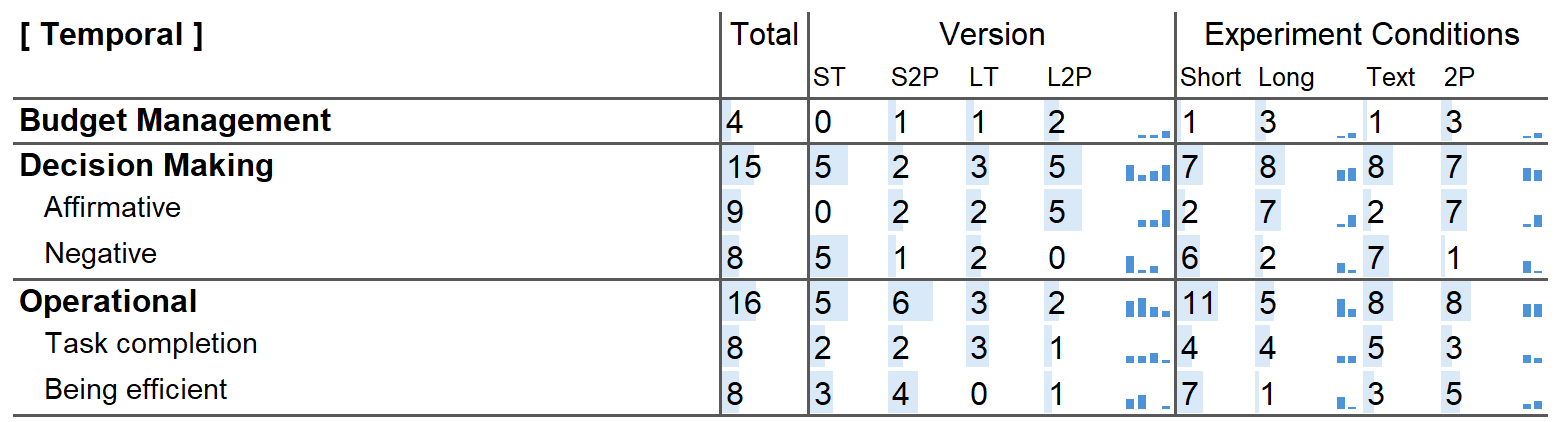
\includegraphics[width=\linewidth]{content/image/cog/temporal_table.png}
\end{table}

\subsection{Source of Temporal Demand} 
\label{sec:temporal}
\vspace{5pt}

\begin{tldrbox}
    \faInfoCircle~\xspace\textbf{Summary:} Participants faced increased temporal demand from: \textit{Budget}, \textit{Decision Complexity}, and \textit{Operational Tasks}. Notably, the interactive interface managed temporal demand more effectively, allowing participants to pace themselves and avoid misperceiving task difficulty.
\end{tldrbox}

Temporal demand measures the time pressure participants feel during a task. Lower demand means a more leisurely pace. The main sources of increased temporal demand are (Table~\ref{tbl:temporal}) of increased temporal demand are:~\textit{Budget}, ~\textit{Decision Complexity}, and ~\textit{Operational Tasks}. 

\subsubsection{Temporal Demand Source: Budget}
Budget emerged as a theme across all conditions, with four participants feeling rushed as their credits decreased, translating the increasing marginal cost of votes into higher temporal demand. As one participant said:

\begin{displayquote}
When the money was decreasing, as I was casting more upvotes or downvotes so as the money decreases I felt kind of rushed.
            
\noindent \hfill -- S034, long interactive interface
\end{displayquote}


\begin{wrapfigure}{r}{0.45\textwidth} % Adjust the width as needed
    \centering
    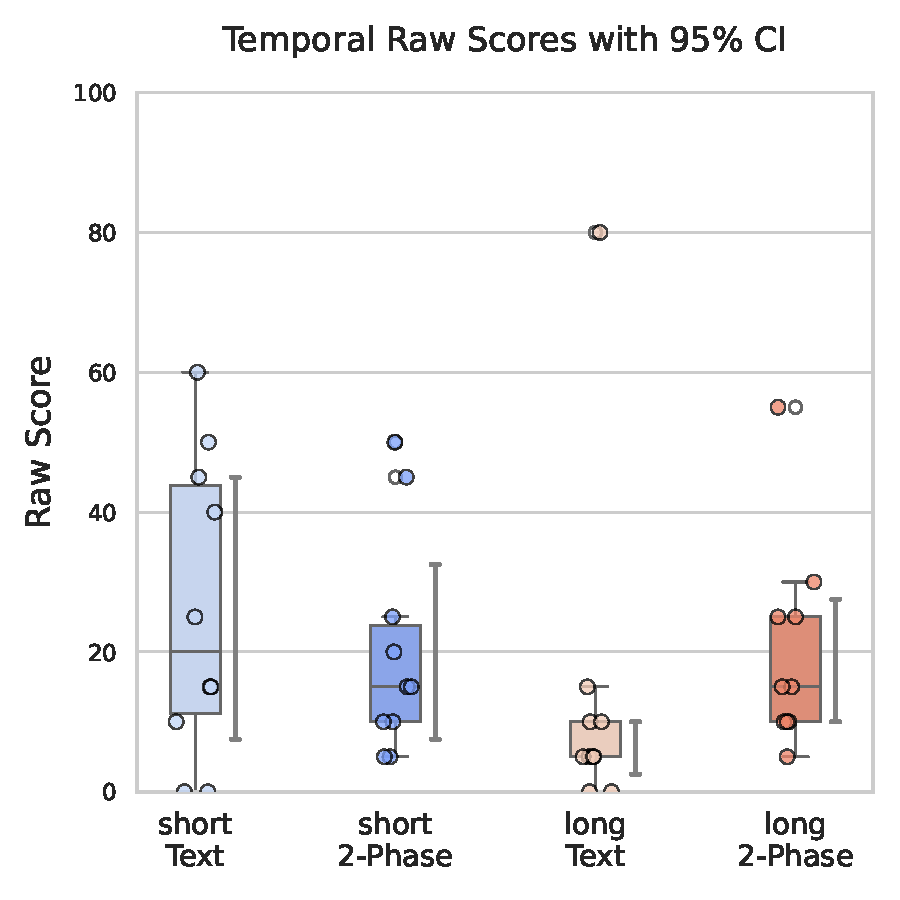
\includegraphics[width=0.45\textwidth, trim=0 13 0 13, clip]{content/image/cog/Temporal_scores.pdf}
    \captionsetup{width=0.40\textwidth, justification=justified} % Adjust the width to match the image width
    \caption{Temporal Demand Raw Score: The short text interface results in the highest temporal demand, while the long text interface has the lowest. Both interactive interfaces, particularly the short interactive, show moderate temporal demand, suggesting that interactive elements help manage time pressure more effectively, allowing participants to pace themselves better and engage more deeply in the tasks.}
    \label{fig:temporal_cog_score}
\end{wrapfigure}

\subsubsection{Temporal Demand Source: Decision Complexity through different lens}
Decision Complexity refers to when participants felt that there are many decisions to make. These causes appear in two forms -- affirmative and negative. Affirmative perception refers to participants explicitly expressing that there are many decisions~\textit{to make}, while negative perception refers to participants describing concerns regarding the time and effort~\textit{already invested} in the survey.

\begin{displayquote}
\bracketellipsis when you are being presented the ideas that they're that they are being put together, and you need to allocate the resources~\ldots Say, you know, this one is more important than that one~\ldots that's the part when it gets tricky, so that you spend more time here. 
    
\noindent \hfill -- S037, long interactive interface
\end{displayquote}

\begin{displayquote}
\bracketellipsis so at first it was like, `Okay, this is fine.' But then on the end, I was like, maybe I should just hurry up and make a decision. So it's like at first it would been here, but then I kinda moved up near the end when I was hanging a waffling between my upvotes.
\noindent \hfill -- S024, short text interface
\end{displayquote}

The first quote illustrates temporal demand from the decisions participants need to make. The second highlights demand from the time already devoted. In the short text interface, half of the participants expressed negative perceptions of temporal demand, whereas in the long interactive interface, half had affirmative perceptions.

\subsubsection{Temporal Demand Source: Operational Tasks}
Operational tasks involve actions like updating votes and completing the survey. For instance, one participant aimed to operate swiftly:

\begin{displayquote}
I wanna get through things in an efficient manner which doesn't necessarily mean I rush it. But it does mean that I do things expeditiously. Especially. I'd like to think I'm somewhat computer-savvy. And so to be able to move through this quickly and efficiently. I do take pride in, but it's all personal stuff. It's not nothing outwardly influencing me. 
        
\noindent \hfill -- S032, short text interface
\end{displayquote}

\begin{displayquote}
I want the credit done but I don't want to be overthinking.
            
\noindent \hfill -- S013, short text interface
\end{displayquote}

The first quote refers to the participant's aim to operate swiftly on the interface, not specifically related to decision making. Similarly, the latter focuses on using the credit to complete a specific goal. We found that temporal demand is higher for the short survey experiment group. Over half of the participants from the short interface wanted to complete the task swiftly and quickly, compared to $5$ participants from the long QS group.

\subsubsection{Takeaway: Temporal demand managed through interactive interface}
The raw NASA-TLX values in Fig~\ref{fig:temporal_cog_score} visually indicate two important points. First, temporal demand trended lower for the interactive interface in the short QS condition, while it trended higher for the long QS condition. Second, the long text interface exhibited the lowest temporal demand, which is counterintuitive since participants in this condition made no fewer decisions and operations compared to the short text group. According to our interpretation of mental demand results in Section~\ref{sec:mental_takeaway}, participants likely did not experience temporal demand because they applied heuristics to reduce the number of decisions, thereby lowering their cognitive load and decision-making instances.

Additionally, participants in the long interactive condition reported that the numerous required operations created temporal demand, preventing them from taking mental shortcuts and shifting their cognitive load to different dimensions.

Furthermore, participants in the short text QS expressed high temporal demand and perceived it negatively, likely misperceiving task difficulty. Conversely, even though the short interactive interface required more decisions, participants reported less temporal demand from decision-making, resulting in a lower overall score. This suggests that the interactive interface slowed them down without increasing temporal demand, allowing them to pace themselves and engage in more in-depth thinking, thereby preventing a misperception of task difficulty.

These observations across experimental conditions support the plausible explanation that the interactive interface mitigated satisficing behaviors due to cognitive overload, as evidenced by the different sources of temporal demand.

%  TODO: move to discussion?
% It is also worth noting that three participants from the 20 who responded to the long survey mentioned that the vertical screen's ability to see all options facilitated direct comparisons and transparency about the entirety of the task, which reduced the temporal demand.

% \begin{displayquote}
% (Seeing) all at once I can see how many there are, so it's kind of like I can kind of tell when I will be done.

% \noindent \hfill -- S041, long text interface
% \end{displayquote}

% ============================================= %
\begin{table}[h]
    \caption{Performance Causes: Most causes are shared across experiment conditions. We provided qualitative interpretations of their own perfornace assessments.}
    \label{tbl:physical}
    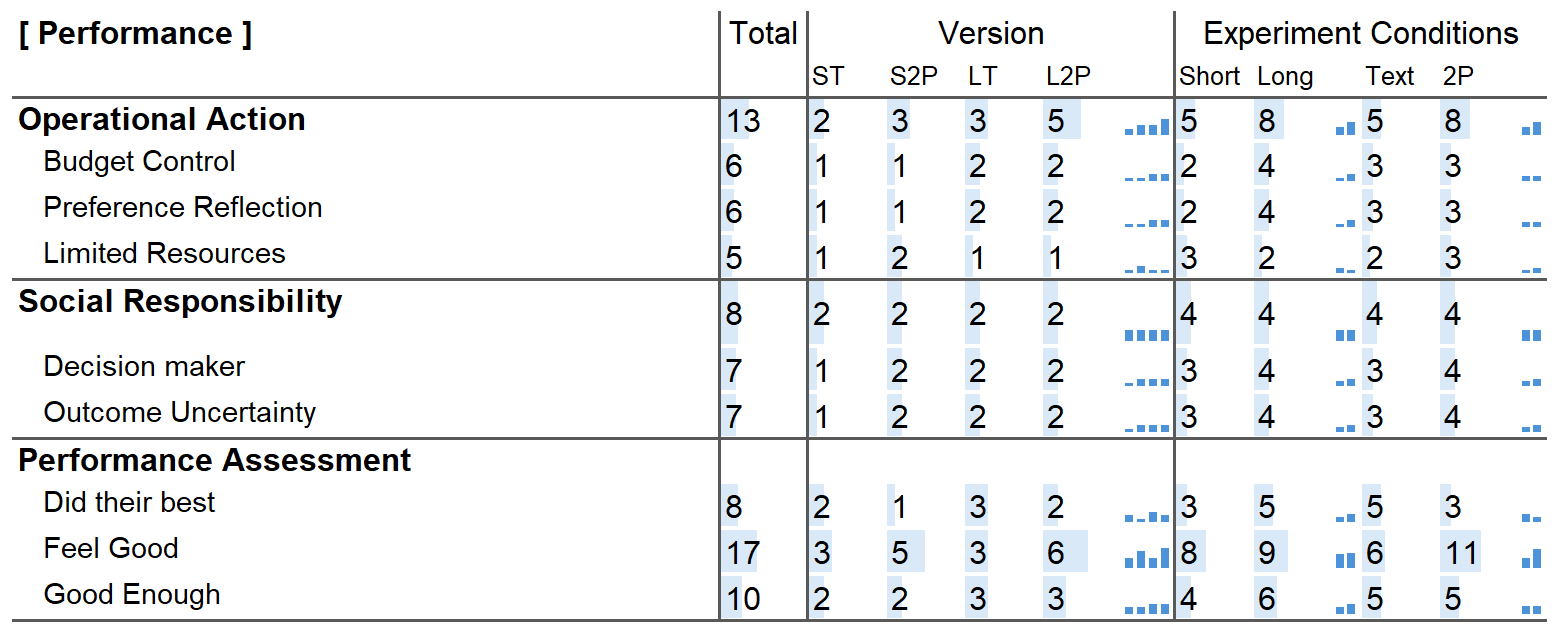
\includegraphics[width=\linewidth]{content/image/cog/perf_table.png}
\end{table}

\subsection{Source of Performance}
\label{sec:performance}
\vspace{5pt}

\begin{tldrbox}
    \faInfoCircle~\xspace\textbf{Summary:} Participants experienced performance demands due to \textit{Operational Actions} and \textit{Social Responsibility}. Despite similar performance scores across groups, more participants using the interactive interface felt more positive about their performance.
\end{tldrbox}

Performance refers to a person's perception of their success in completing a task. Lower values mean good performance; higher values mean poor performance. We found minimal qualitative differences between experiment groups regarding influence sources. We identified two performance demands from the interviews: \textit{Operational Actions} and \textit{Social Responsibility}. Despite most participants reporting positively on their performance, nuances exist in how different groups interpret their performance.

\subsubsection{Performance Source: Operational Actions}
Operational actions, like the theme presented in temporal demand, refer to specific, executable procedures participants perform in the survey. All experiment groups share these sources. Six participants felt pressured to spend all their credits or stay within budget. Five participants worried choice of votes didn't reflect their true preferences. Additionally, six participants experienced performance demand due to limited time, energy, and resources, which ties into other specific cognitive demands like decision fatigue and time pressure. Here we show two examples:

\begin{wrapfigure}{r}{0.45\textwidth} % Adjust the width as needed
    \centering
    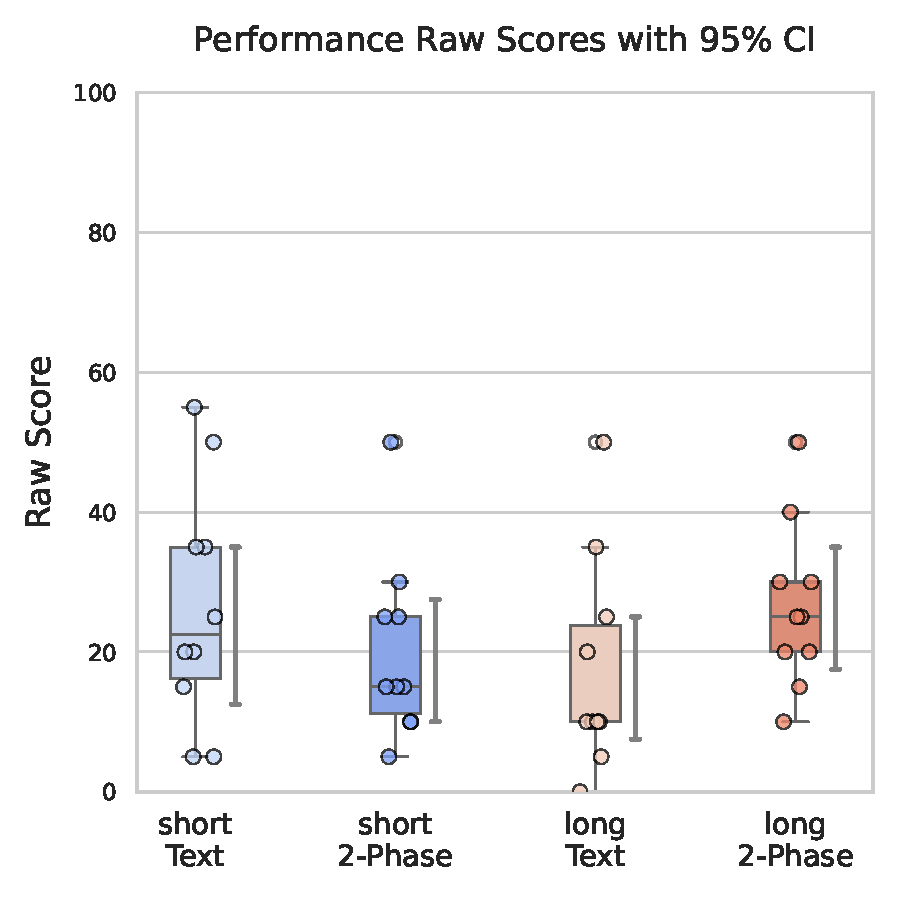
\includegraphics[width=0.45\textwidth, trim=0 13 0 13, clip]{content/image/cog/Performance_scores.pdf}
    \captionsetup{width=0.40\textwidth, justification=justified} % Adjust the width to match the image width
    \caption{Performance Demand Raw Score: Participants showed indifferent performance raw scores across experiment conditions, all trending toward satisfactory.}
    \label{fig:performance_cog_score}
\end{wrapfigure}

\begin{displayquote}
I don't think I did it perfectly, because I didn't have 0 remaining credits.
    
\noindent \hfill -- S024, short text interface, budget management
\end{displayquote}

\begin{displayquote}
I'm concerned that it's not as reflective of my views as I wanted to be like, or I was concerned about it.~\bracketellipsis I was concerned that maybe it didn't.

\noindent \hfill -- S041, long text interface, preference reflectiveness
\end{displayquote}


\subsubsection{Performance Source: Social Responsibility}
Social Responsibility is a noteworthy performance demand, categorized into \textit{decision-maker responsibility} (N=8) and \textit{uncertainty of the outcome} (N=3). The former refers to individuals feeling guilty because they couldn’t avoid specific tradeoffs or wanted to be fair. This theme resembles `External Demand' in Mental Demand. For example,

\begin{displayquote}
I don't want people to think that I just like don't care about <ethnicity> people at all. I also don't think like government funding should go towards like religious organizations. You know what I mean. So I don't want somebody to think that like, I just don't care about <ethnicity> people.
    
\noindent \hfill -- S041, long text interface, decision-maker responsibility
\end{displayquote}

In this quote, the participant put themselves inside the shoes of a member of the government, rather than a citizen expressing their own attitudes. This shift in roles introduced the performance demand and demonstrated that QS mirrors the decision-maker's dilemma in individual survey responses. This characteristic also applies to the latter, further highlighting participants' attempts to foresee an outcome:

\begin{displayquote}
If I was actually running a government funding~\bracketellipsis I don't know how this (the survey results) might actually affect people. Some of these things might be unpopular or bad, or have outcomes that I didn't forsee.
    
\noindent \hfill -- S027, short interactive interface, uncertainity of the outcome
\end{displayquote}

Social responsibility also spans experiment groups. Raw NASA-TLX scores (Figure~\ref{fig:performance_cog_score}) show participants had indistinguishable performance scores. This aligns with the interview results where most participants felt positive about their final submission. We also analyzed participants' satisfactory statements regarding performance.

\subsubsection{Takeaway: Half of the participants using the interactive interface~\textit{Felt good}}
We identified three types of satisfactory statements regarding self-reported performance:
\begin{itemize}
    \item \textit{Did their best} refers to statements where a participant stated they exhausted their maximum effort to complete the task.
    \item \textit{Feel good} refers to statements where a participant expressed positive emotions or satisfaction about their performance or the outcome.
    \item \textit{Good enough} refers to statements where a participant acknowledged that their performance or the outcome was acceptable or satisfactory, but not necessarily perfect or the best possible.
\end{itemize}

Approximately the same number of participants in each of the four experiment groups expressed \textit{Good enough}. Meanwhile, participants using the interactive interface across short and long groups had almost double the number of participants ($N=11$) who expressed \textit{Feel good} compared to the text interface ($N=6$).The text interface had slightly more participants ($N=5$) who expressed \textit{Did their best} compared to the interactive interface ($N=3$).

These results highlight key takeaways: First, participants from all experiment groups expressed satisficing behaviors (\textit{Good enough}) at similar frequencies. Second, participants using the interactive interface were generally more positive about their experience and the outcomes.

% TODO: Need to check the reflective thinking part a bit. I **think** there are differences but it is unclear, need to go back to raw code.


% ============================================= %
\begin{table}[h]
    \caption{Mental Demand Sources: Participants using the text interface focused more on operational tasks, while those using the interactive interface focused more on strategic planning.}
    \label{tbl:physical}
    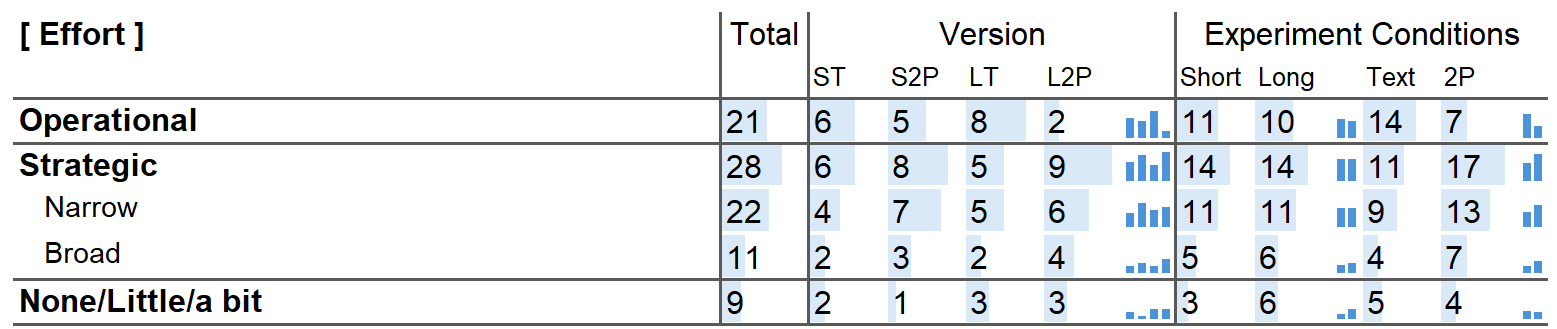
\includegraphics[width=\linewidth]{content/image/cog/effort_table.png}
\end{table}

\subsection{Source of Effort}
\label{sec:effort}

\vspace{5pt}
\begin{tldrbox}
    \faInfoCircle~\xspace\textbf{Summary:} Effort sources varied between operational~\textit{Operational Tasks} and~\textit{Strategic Planning}. Participants using the text interface focused on operational tasks, while those using the interactive interface engaged in strategic planning. This shows that the interactive interface spurs deeper, more critical thinking.
\end{tldrbox}
Effort refers to work required to achieve a level of performance. It includes the intensity of both mental and physical resources expended during the task. We identified two major sources of effort: \textit{Operational Tasks} and \textit{Strategic Planning}.

\subsubsection{Effort Source: Operational Tasks} Operational Tasks that increase effort includes navigating the interface, managing the budget at an operational scale (i.e., making sure not to run out of budget, making specific updates between two options), or translating opinions into quantifiable adjustment on the survey, all directly related to manipulating the interface. We show two examples:

\begin{displayquote}
And then I wanted to bump up (an option) maybe to 4 or <option> to 5 and realize I couldn't. My point (number of votes) had to like back down a little bit~\ldots So that would be effort came in of how do I want to really rearrange this to make it (the budget spending) maximize?

\noindent \hfill -- S029, short text interface
\end{displayquote}

\begin{displayquote}
So it was like it was very~\ldots I have to put a lot of effort in terms of you know~\ldots think about each dimension that if I give one credit to <option name> whether it will affect my credits on <another option name>.

\noindent \hfill -- S005, long text interface
\end{displayquote}

Both quotes illustrated participants putting in effort to manipulate the interface. $14$ of the $20$ participants using the text interface mentioned these effort sources, compared to $7$ using the interactive interface, with the lowest mention by the long interactive interface group ($N=2$).


\begin{wrapfigure}{r}{0.45\textwidth} % Adjust the width as needed
    \centering
    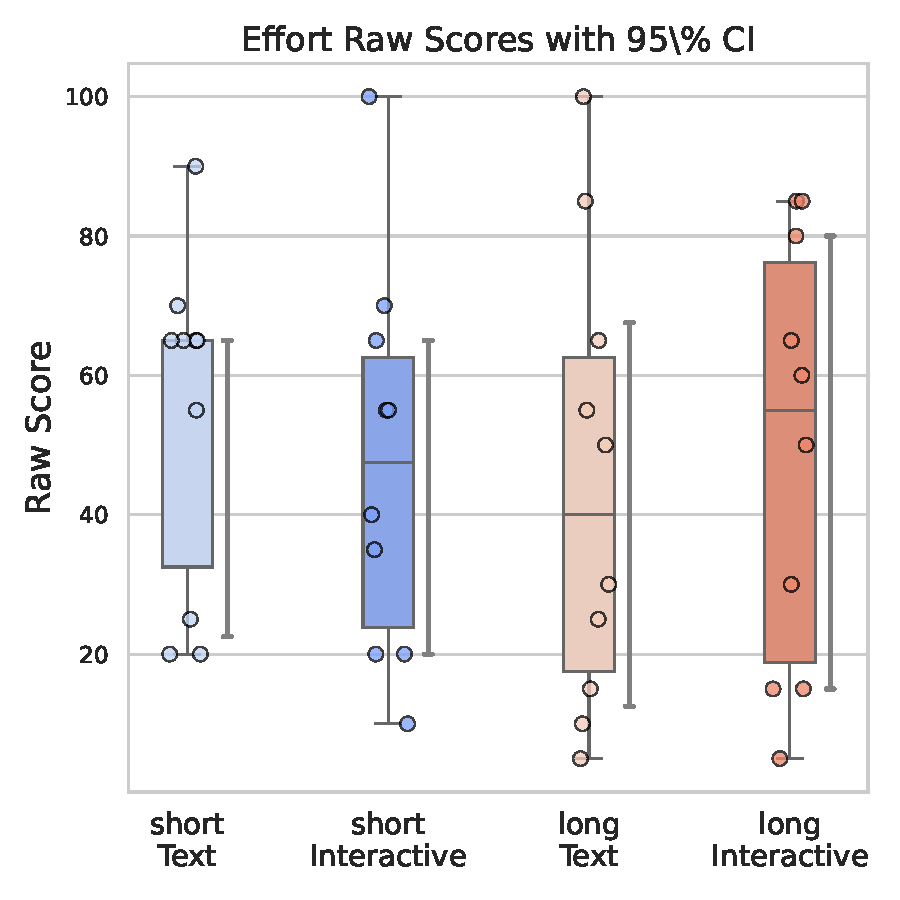
\includegraphics[width=0.45\textwidth, trim=0 13 0 13, clip]{content/image/cog/Effort_scores.pdf}
    \captionsetup{width=0.40\textwidth, justification=justified} % Adjust the width to match the image width
    \caption{Effort Raw Score: Effort scores shows indifference across groups.}
    \label{fig:effort_cog_score}
\end{wrapfigure}


\subsubsection{Effort Source: Strategic Planning}
Strategic planning is similar to strategic budget management mentioned under mental demand. Unlike operational tasks, strategic planning involves higher-level strategies to complete the survey. We categorize two distinct types of planning: \textit{personal} and \textit{global}. \textit{Personal strategic planning} involves translating preferences onto the survey without considering broader values or beliefs. For example:

\begin{displayquote}
~\bracketellipsis having that prior experience and being able to quickly link it to a tangible thing that I've experienced in my personal life.

\noindent \hfill -- S032, short text interface
\end{displayquote}

\begin{displayquote}
And really the bulk of the effort was how to rank order these (options) and allocate the resources behind the upvotes so that I can accurately depict what I want~\ldots say, a committee to focus on and allocate actual fungible resources, too. 

\noindent \hfill -- S019, long interactive interface
\end{displayquote}

Participants using the interactive interface ($N=13$) mentioned personal strategic planning slightly more than those using the text interface ($N=9$). \textit{Global strategic planning}, on the other hand, involves formulating strategies to align with broader communal values, such as fairness and community impact. For example:

\begin{displayquote}
I think, imagining the trying to imagine every outcome trying to to imagine what what else would be encompassed, encompassed by each category.

\noindent \hfill -- S027, short interactive interface
\end{displayquote}

\begin{displayquote}
Hey, even though I don't really like this idea. But what if they're important? They sort of kind of deserve some attention~\ldots that's why I think I have the effort here.

\noindent \hfill -- S037, long interactive interface
\end{displayquote}
    
Both examples show considerations beyond personal experiences, including outcomes or social values. Nearly twice as many participants using the interactive interface ($N=7$) mentioned global strategic efforts compared to the text interface ($N=4$). Overall, more participants using the interactive interface ($N=17$) reported sources of strategic effort compared to those using text-based interfaces ($N=11$).

\subsubsection{Takeaway: Interactive interface spurs more strategic effort from participants}
Effort is a realization of mental demand through physical actions. Since participants experienced little physical demand, the sources of effort reflected how individuals translated their mental demand into efforts. The raw NASA-TLX effort scores (Figure~\ref{fig:effort_cog_score}) showed a similar spread across experiment groups, akin to mental demand. However, qualitative analysis revealed that participants using the text interface experienced more effort focused on operational tasks (i.e., completing specific tasks). In contrast, participants using the interactive interface experienced more effort focused on strategic planning (planning a strategy to complete tasks). Specifically, those using the interactive interface engaged in global strategic planning, considering options comprehensively and beyond the immediate task. This contrasts with text interface participants, who concentrated more on operational tasks and narrower strategic planning. This finding reinforces that cognitive load sources differ between interfaces, with interactive interfaces fostering deeper, more critical thinking.

% ============================================= %
\begin{table}[h]
    \caption{Fustration Sources: needs to be updated with some new terms definitions for some of the columns.}
    \label{tbl:fustration}
    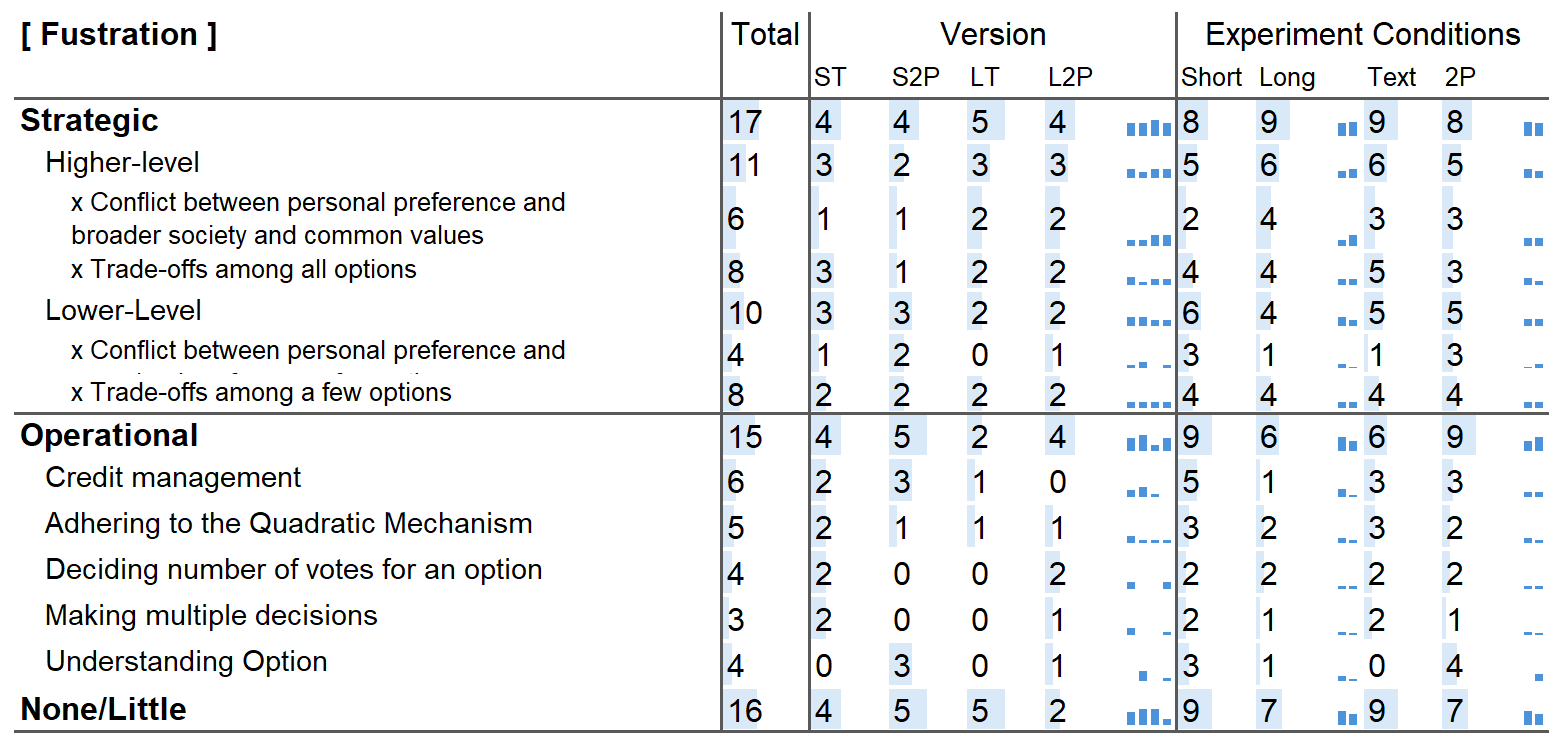
\includegraphics[width=\linewidth]{content/image/cog/fustration_table.png}
\end{table}
\subsection{Source of Fustration} 
\label{sec:fustration}

\vspace{5pt}
\begin{tldrbox}
    \faInfoCircle~\xspace\textbf{Summary:} Participants experienced frustration from two main sources: \textit{Operational Actions} and \textit{Strategic Planning}. We observed evidence that participants in the long text interface showed little fustration, specifically from operational sources, indicating satisficing behaviors.
\end{tldrbox}

Frustration refers to the extent to which the participant is annoyed, irritated, or discouraged during the task. Sources of frustration are grouped into two major themes: \textit{Operational Actions} and \textit{Strategic Planning}.

\subsubsection{Operational Actions} 
$15$ participants highlighted this source for frustration. $6$ participants expressed frustration regarding credit management (i.e., overspending budget); $4$ participants mentioned had trouble deciding the final value for the options; $3$ participants are frustrated because they need to make multiple decisions; $5$ participants were frustrated with the quadratic mechanism; $4$ participants are frustrated trying to understand the content of the option or how the option connects to them. For example, 

\begin{displayquote}
I was slightly frustrated when doing the task, probably because there was a budget that we kind of had to stick with it.

\noindent \hfill -- S001, long text interface, quadratic mechanism
\end{displayquote}

\begin{displayquote}
i think just frustration~\bracketellipsis because when i was making like the decisions on how many upvotes I could put in each section, I was running out of credits.

\noindent \hfill -- S013, short interactive interface, budget management
\end{displayquote}

These demonstrate participants' frustration when hindered by operational actions or constraints presented by QS. Notably, almost half of the participants in all experiment groups expressed operational frustration, compared to only two participants from the long text interface group.

\begin{wrapfigure}{r}{0.45\textwidth} % Adjust the width as needed
    \centering
    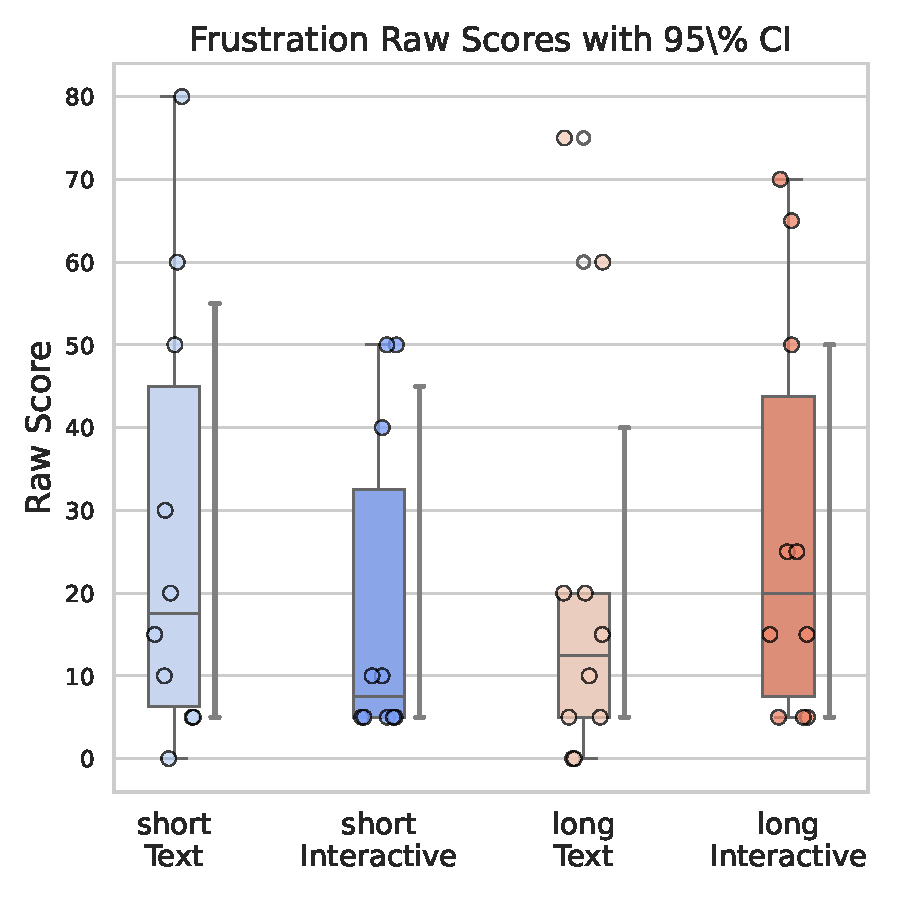
\includegraphics[width=0.45\textwidth, trim=0 13 0 13, clip]{content/image/cog/Frustration_scores.pdf}
    \captionsetup{width=0.40\textwidth, justification=justified} % Adjust the width to match the image width
    \caption{Fustration Raw Score: Participants other than the long text interface highlighted seversl operational tasks that led to fustration. All groups share causes from strategic planning.}
    \label{fig:fustration_cog_score}
\end{wrapfigure}

\subsubsection{Strategic Planning}
We derived strategic planning into two types: \textit{lower-level} and \textit{higher-level}. Four participants experienced conflict between their own and others' preferences. Eight participants experienced conflict when making trade-offs among a few options. For example:

\begin{displayquote}
Because I know that's important to other people. But it just doesn't to me.
    
\noindent \hfill -- S010, short interactive interface
\end{displayquote}

\begin{displayquote}
I would have loved to have given more to other groups~\ldots and I felt stressed like~\bracketellipsis well~\ldots it's a group that you know is still~\ldots you know~\ldots important~\bracketellipsis
\noindent \hfill -- S020, long text interface
\end{displayquote}

These quotes show participants adhering to lower-level strategies like balancing personal preferences and smaller trade-offs. Compared to~\textit{higher-level strategic planning}, $6$ participants expressed conflicts involving broader societal concerns and core values. $8$ participants felt frustrated by being forced to make trade-offs among~\textit{all} options. For example,

\begin{displayquote}
I had to consider how I feel towards that~\ldots how religious media broadcasting is being used in like today's society~\ldots today's political environment. So yeah~\ldots you really have to consider what is important to you. 
\noindent \hfill -- S020, long text interface, value conflicts
\end{displayquote}

\begin{displayquote}
I think the frustration is~\ldots I wish that we could help all of these causes, but you know it's just like anything else. You can't do everything and when it's not~\ldots  I feel like it's hard to quantify how much some of these things should be supported versus others. So when you're talking about upvotes and things that's challenging to me, it's frustrating.
\noindent \hfill -- S026, long interactive interface, considering all options
\end{displayquote}

All experimental conditions noted similar frustration related to strategy planning, across lower-level and higher-level frustration.

\subsubsection{Takeaway: Long text interface exhibits choice overload evidence}
Across all experimental conditions, participants experience similar sources related to strategic planning. The long text interface condition had the fewest participants expressing operational frustration, with half expressing no frustration. Similar trends appear in the raw NASA-TLX scores (Figure~\ref{fig: fustration_cog_score}), where participants in the long text interface exhibit a much lower frustration score. Both qualitative interview and NASA-TLX scores align with prior literature~\cite{polmanWhyAreMaximizers2010, schwartzMaximizingSatisficingHappiness2002}, indicating that satisficers tend to be less frustrated and happier than maximizers. This suggests that participants in the long text interface exhibit satisficing behaviors, further supporting our claim that the interactive interface can reduce satisficing behaviors in QS tasks.

\subsection{Summary: Interactive interface prevents satisficing, especially for long QS}
We find evidence across all six dimensions contributing to cognitive load that supports the claim that the \textbf{interactive interface prevents satisficing due to cognitive overload}. Evidence from mental demand shows that in the long interactive interface, participants focused more on deeper thinking and were less burdened by precisely determining the number of votes for a few options. Participants using the interactive interface paced themselves better and felt more positive about their performance. Participants devoted more effort, leading to deeper and more critical thinking when using the interactive interface. Participants using the long text interface engaged in satisficing. Despite not seeing drastic differences in the weighted NASA-TLX results and being unable to show strong evidence that the interactive interface is necessary for short QS, our qualitative analysis reveals why long QS need an interactive interface.

In the next section, we further triangulate our hypothesis by examining participant behavior data to show how participants in the long interactive interface behave differently than those in the short interactive interface.



% \begin{figure}[ht]
%     \centering
%     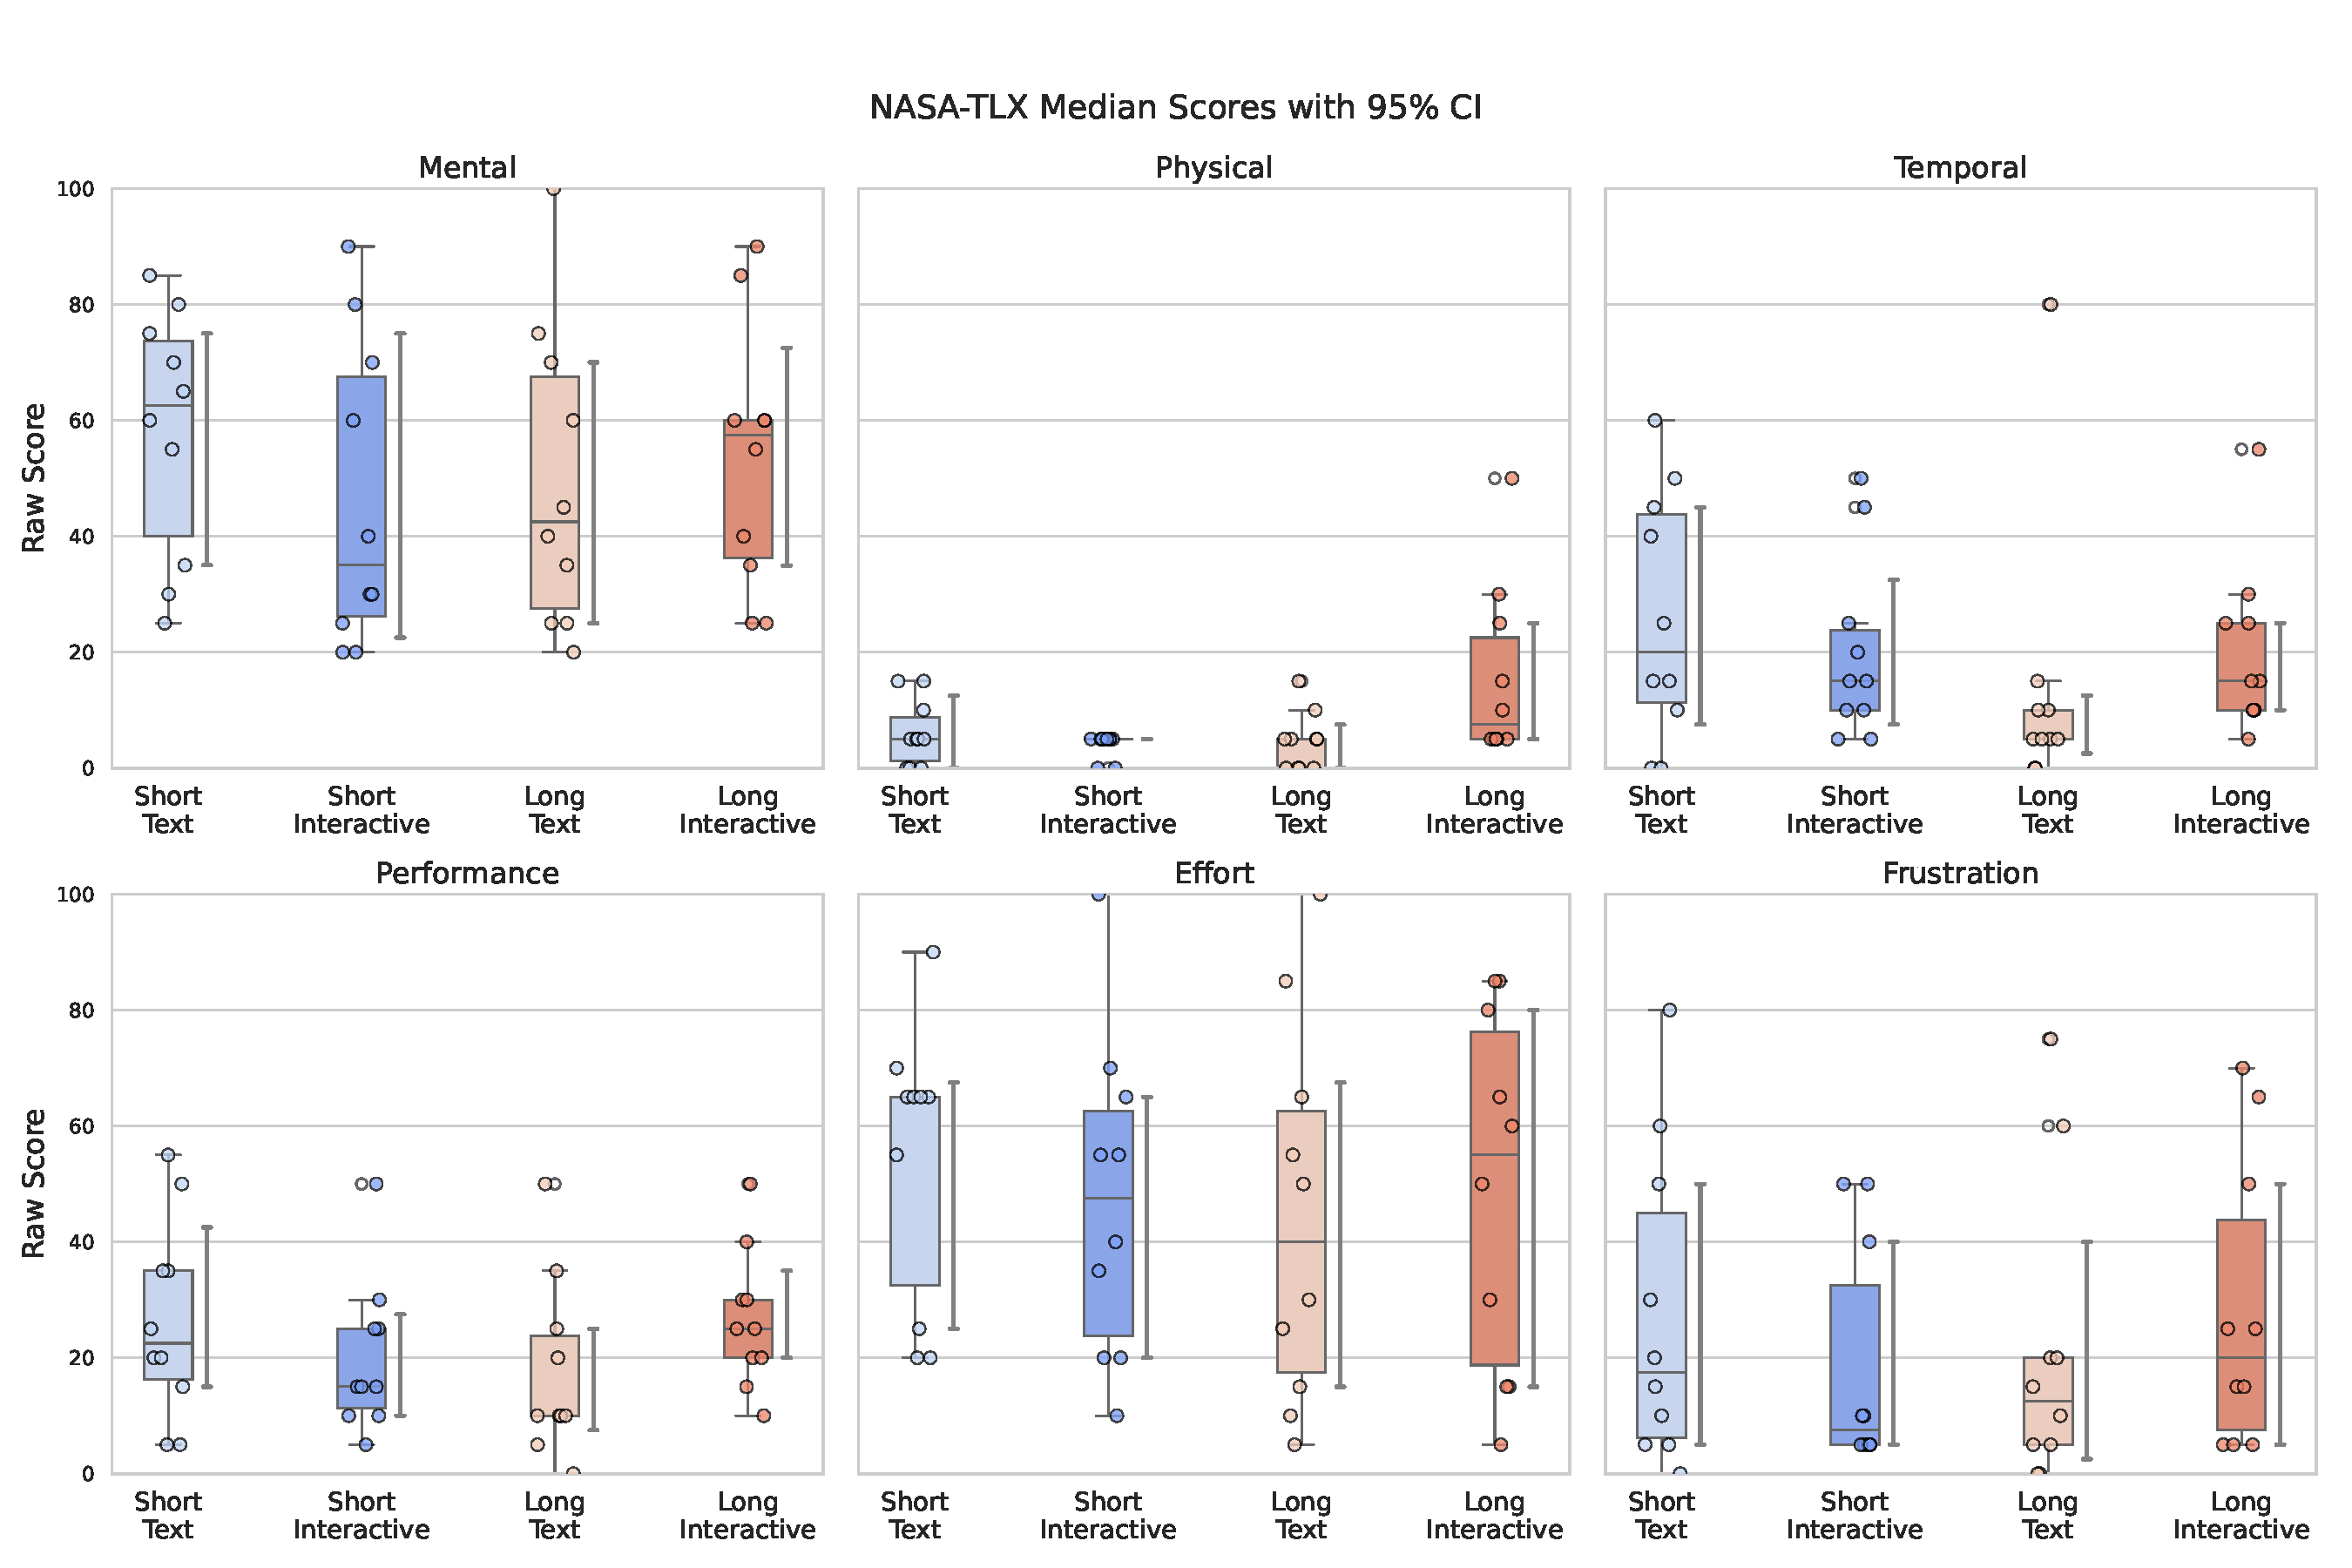
\includegraphics[width=\textwidth]{content/image/cog/nasatlx_final_value_with_CI.pdf}
%     \caption{NASA-TLX Results}
%     \label{fig:nasatlx-with-ci}
% \end{figure}